%%%%%%%%%%%%%%%%%%%%%%%%%%%%%%%%%%%%
% Figures
%%%%%%%%%%%%%%%%%%%%%%%%%%%%%%%%%%%%

% Figure 1
\newcommand{\subFigWidth}{0.50}

\begin{figure}[htbp]
    \centering
    \caption{Timing of Waiting Period Policy Adoption Across All States}
    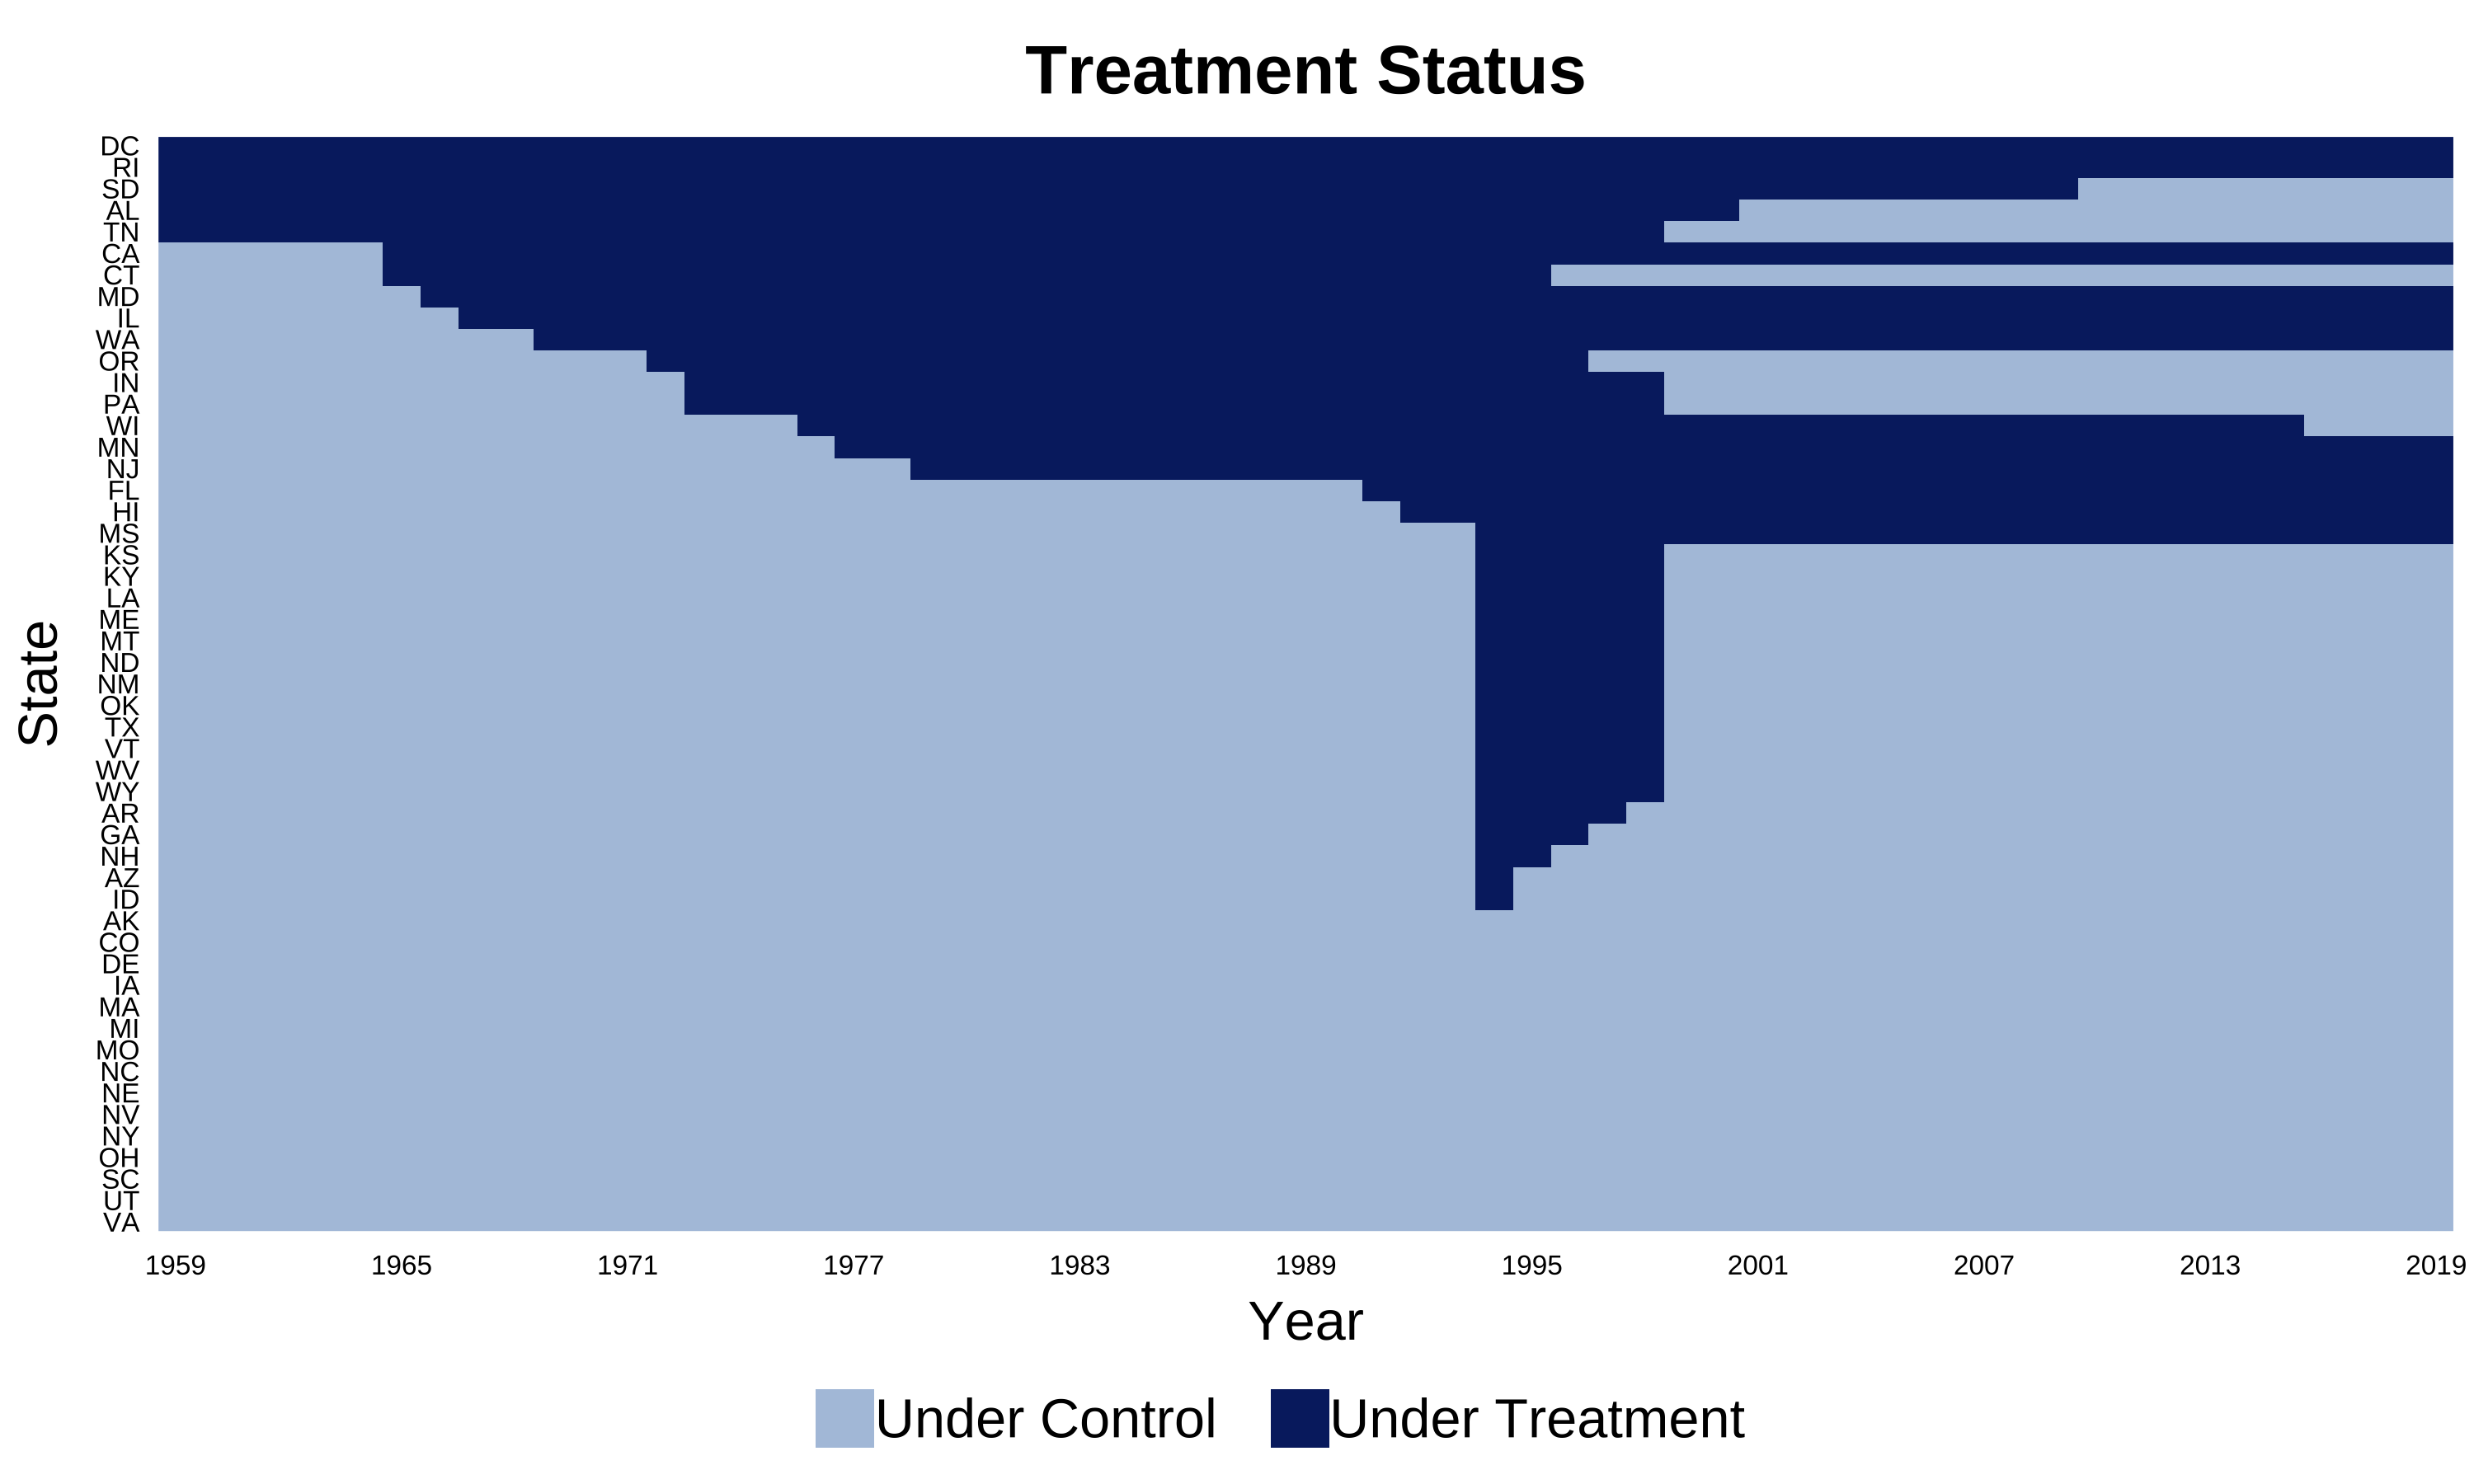
\includegraphics[width=0.8\textwidth]{figures/211-county_year_panel_view}
    \label{fig:211-county_year_panel_vieww}

    \begin{minipage}{\linewidth}
    \caption*{\footnotesize{
      \noindent\textit{Note:} This staggered adoption panel view illustrates the year of waiting period policy implementation or exit for each state. It provides visual clarity on treatment timing across states, which is crucial for interpreting the event study estimates and understanding the source of identifying variation.\\
    \noindent\textit{Source:} RAND State Firearm Law Database, 1813–2015.
 
    }}
  \end{minipage}
\end{figure}


\pagebreak
\clearpage
\begin{figure}[htbp]
    \centering
    \caption{Timing of Waiting Period Policy Adoption Across States}
    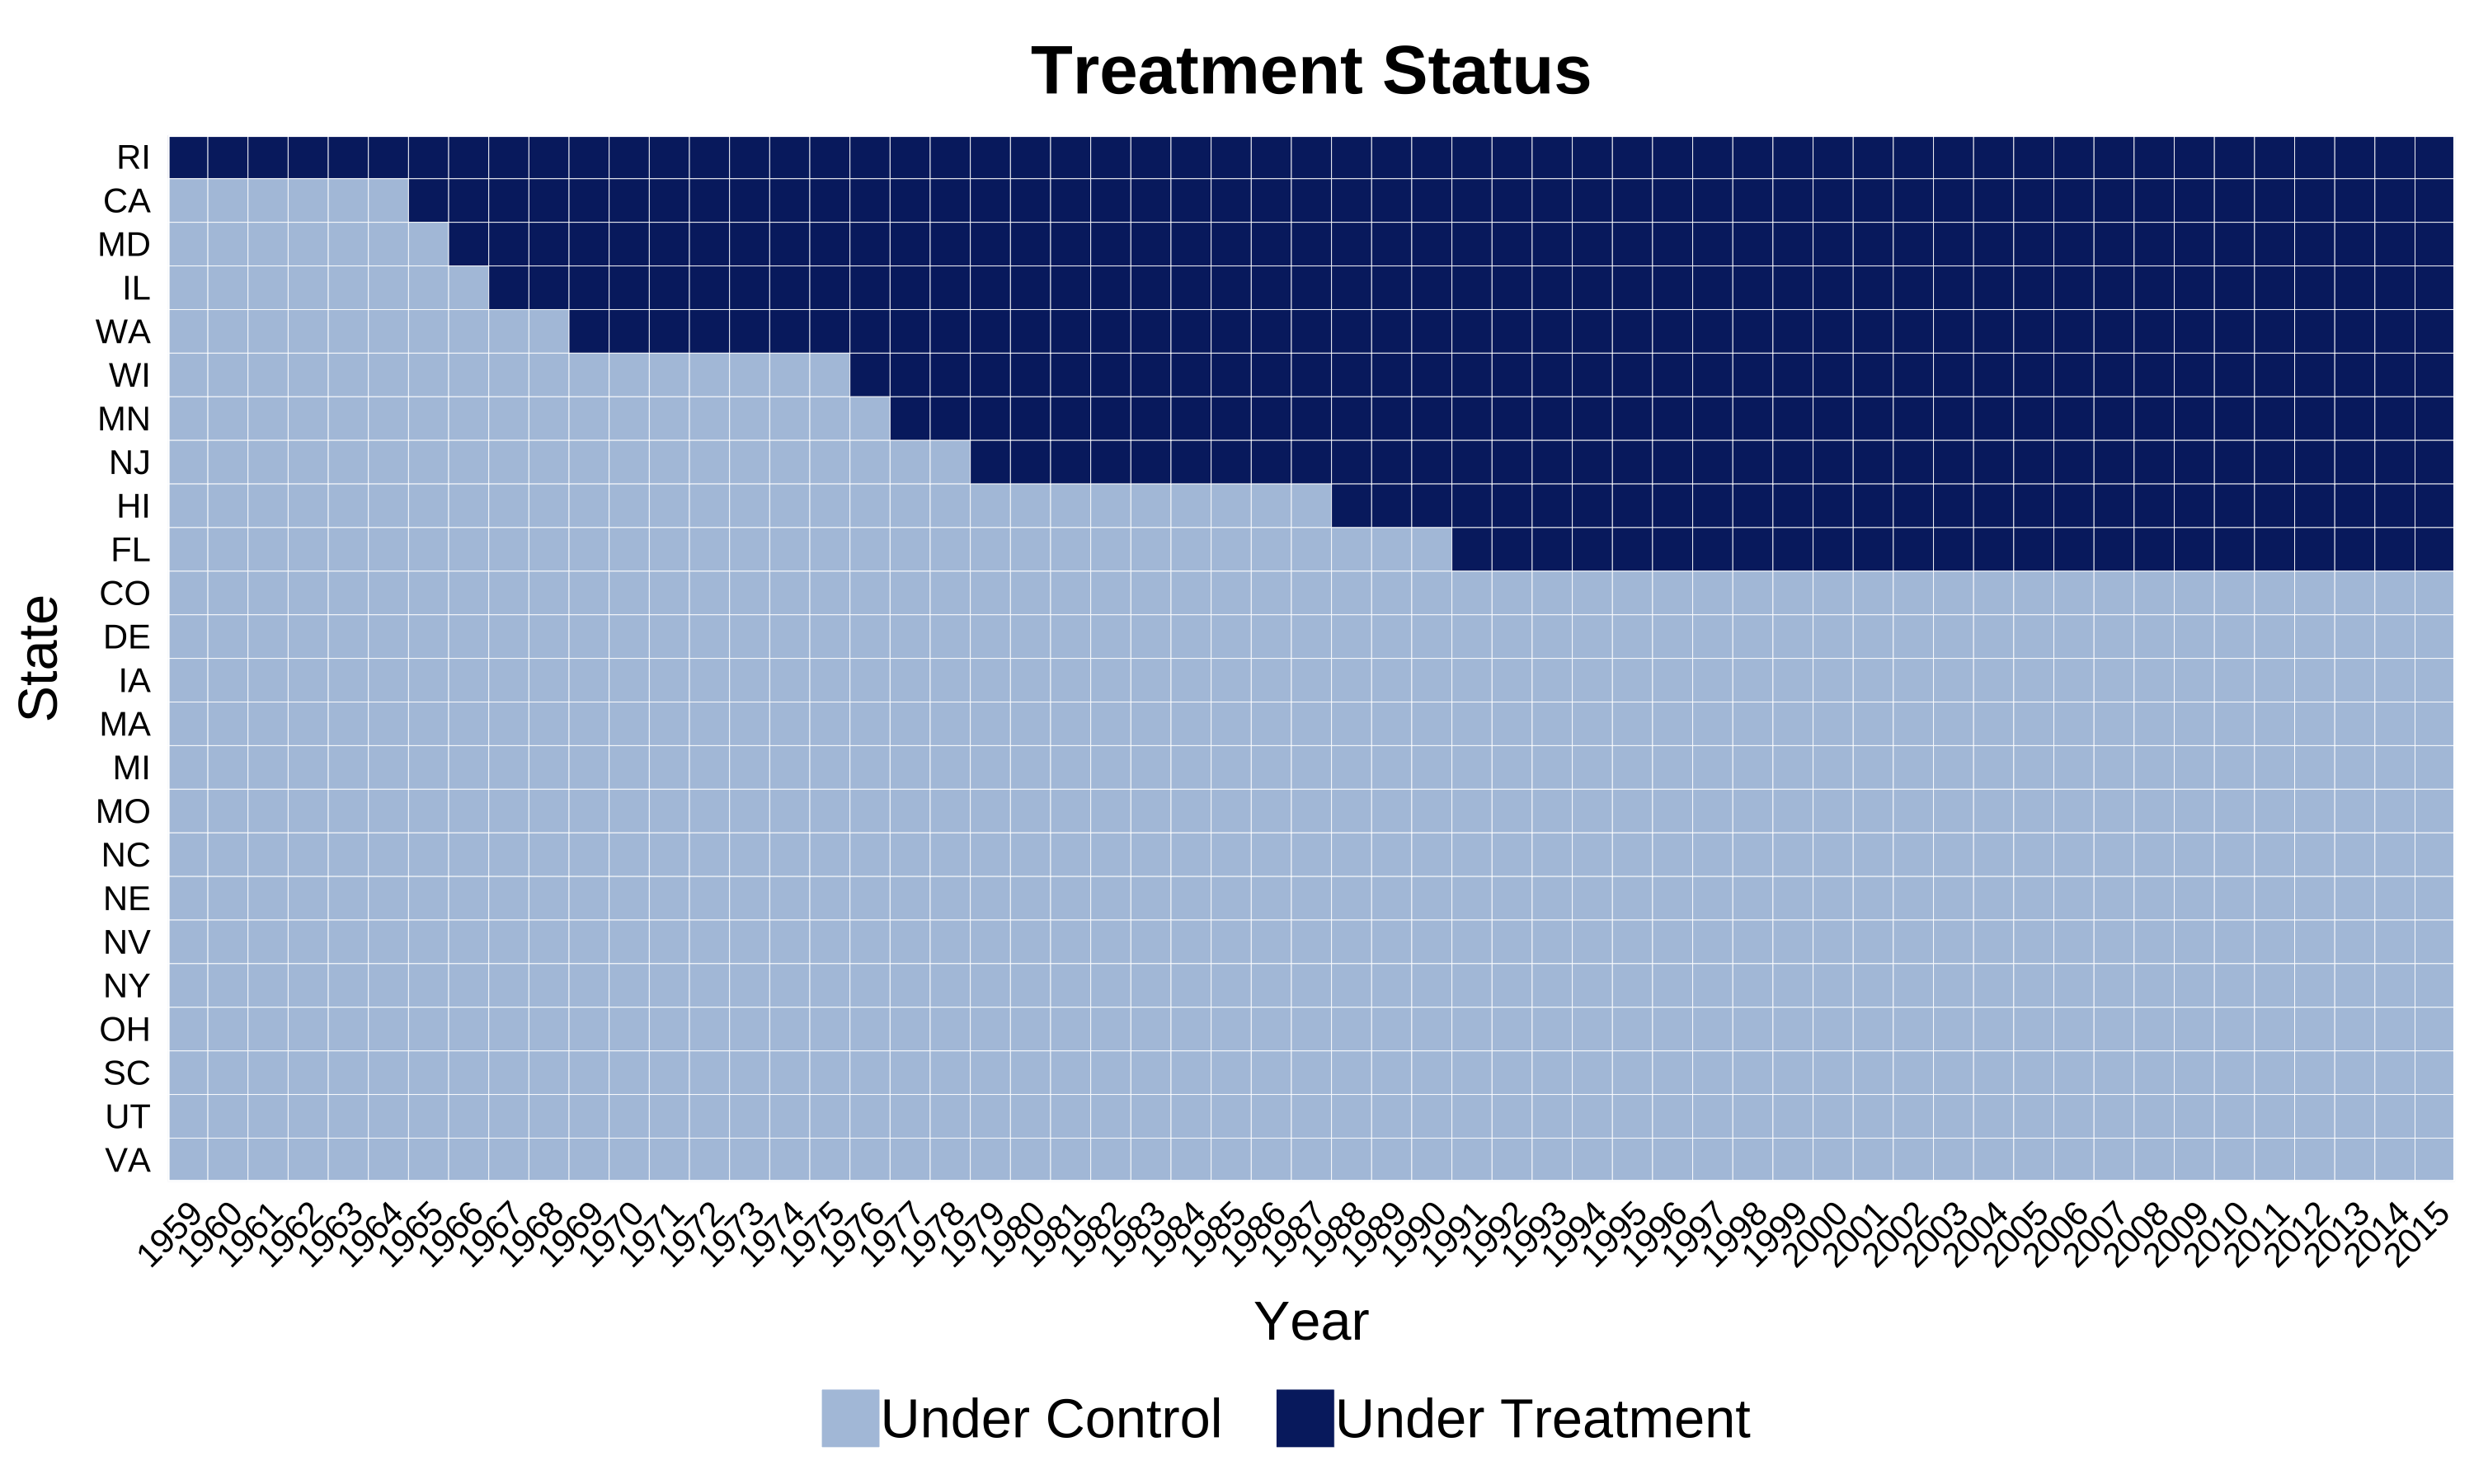
\includegraphics[width=0.8\textwidth]{figures/192-staggarred_sample_panel_view.png}
    \label{fig:192-staggarred_sample_panel_view}

    \begin{minipage}{\linewidth}
    \caption*{\footnotesize{
      \noindent\textit{Note:} This staggered adoption panel view illustrates the year of waiting period policy implementation for each state included in the study. It provides visual clarity on treatment timing across states, which is crucial for interpreting the event study estimates and understanding the source of identifying variation.\\
    \noindent\textit{Source:} RAND State Firearm Law Database, 1813–2015.
 
    }}
  \end{minipage}
\end{figure}


\pagebreak
\clearpage

\begin{figure}[htbp]
    \centering
    \caption{Timing of Waiting Period Policy Adoption Across States: Number of Counties}    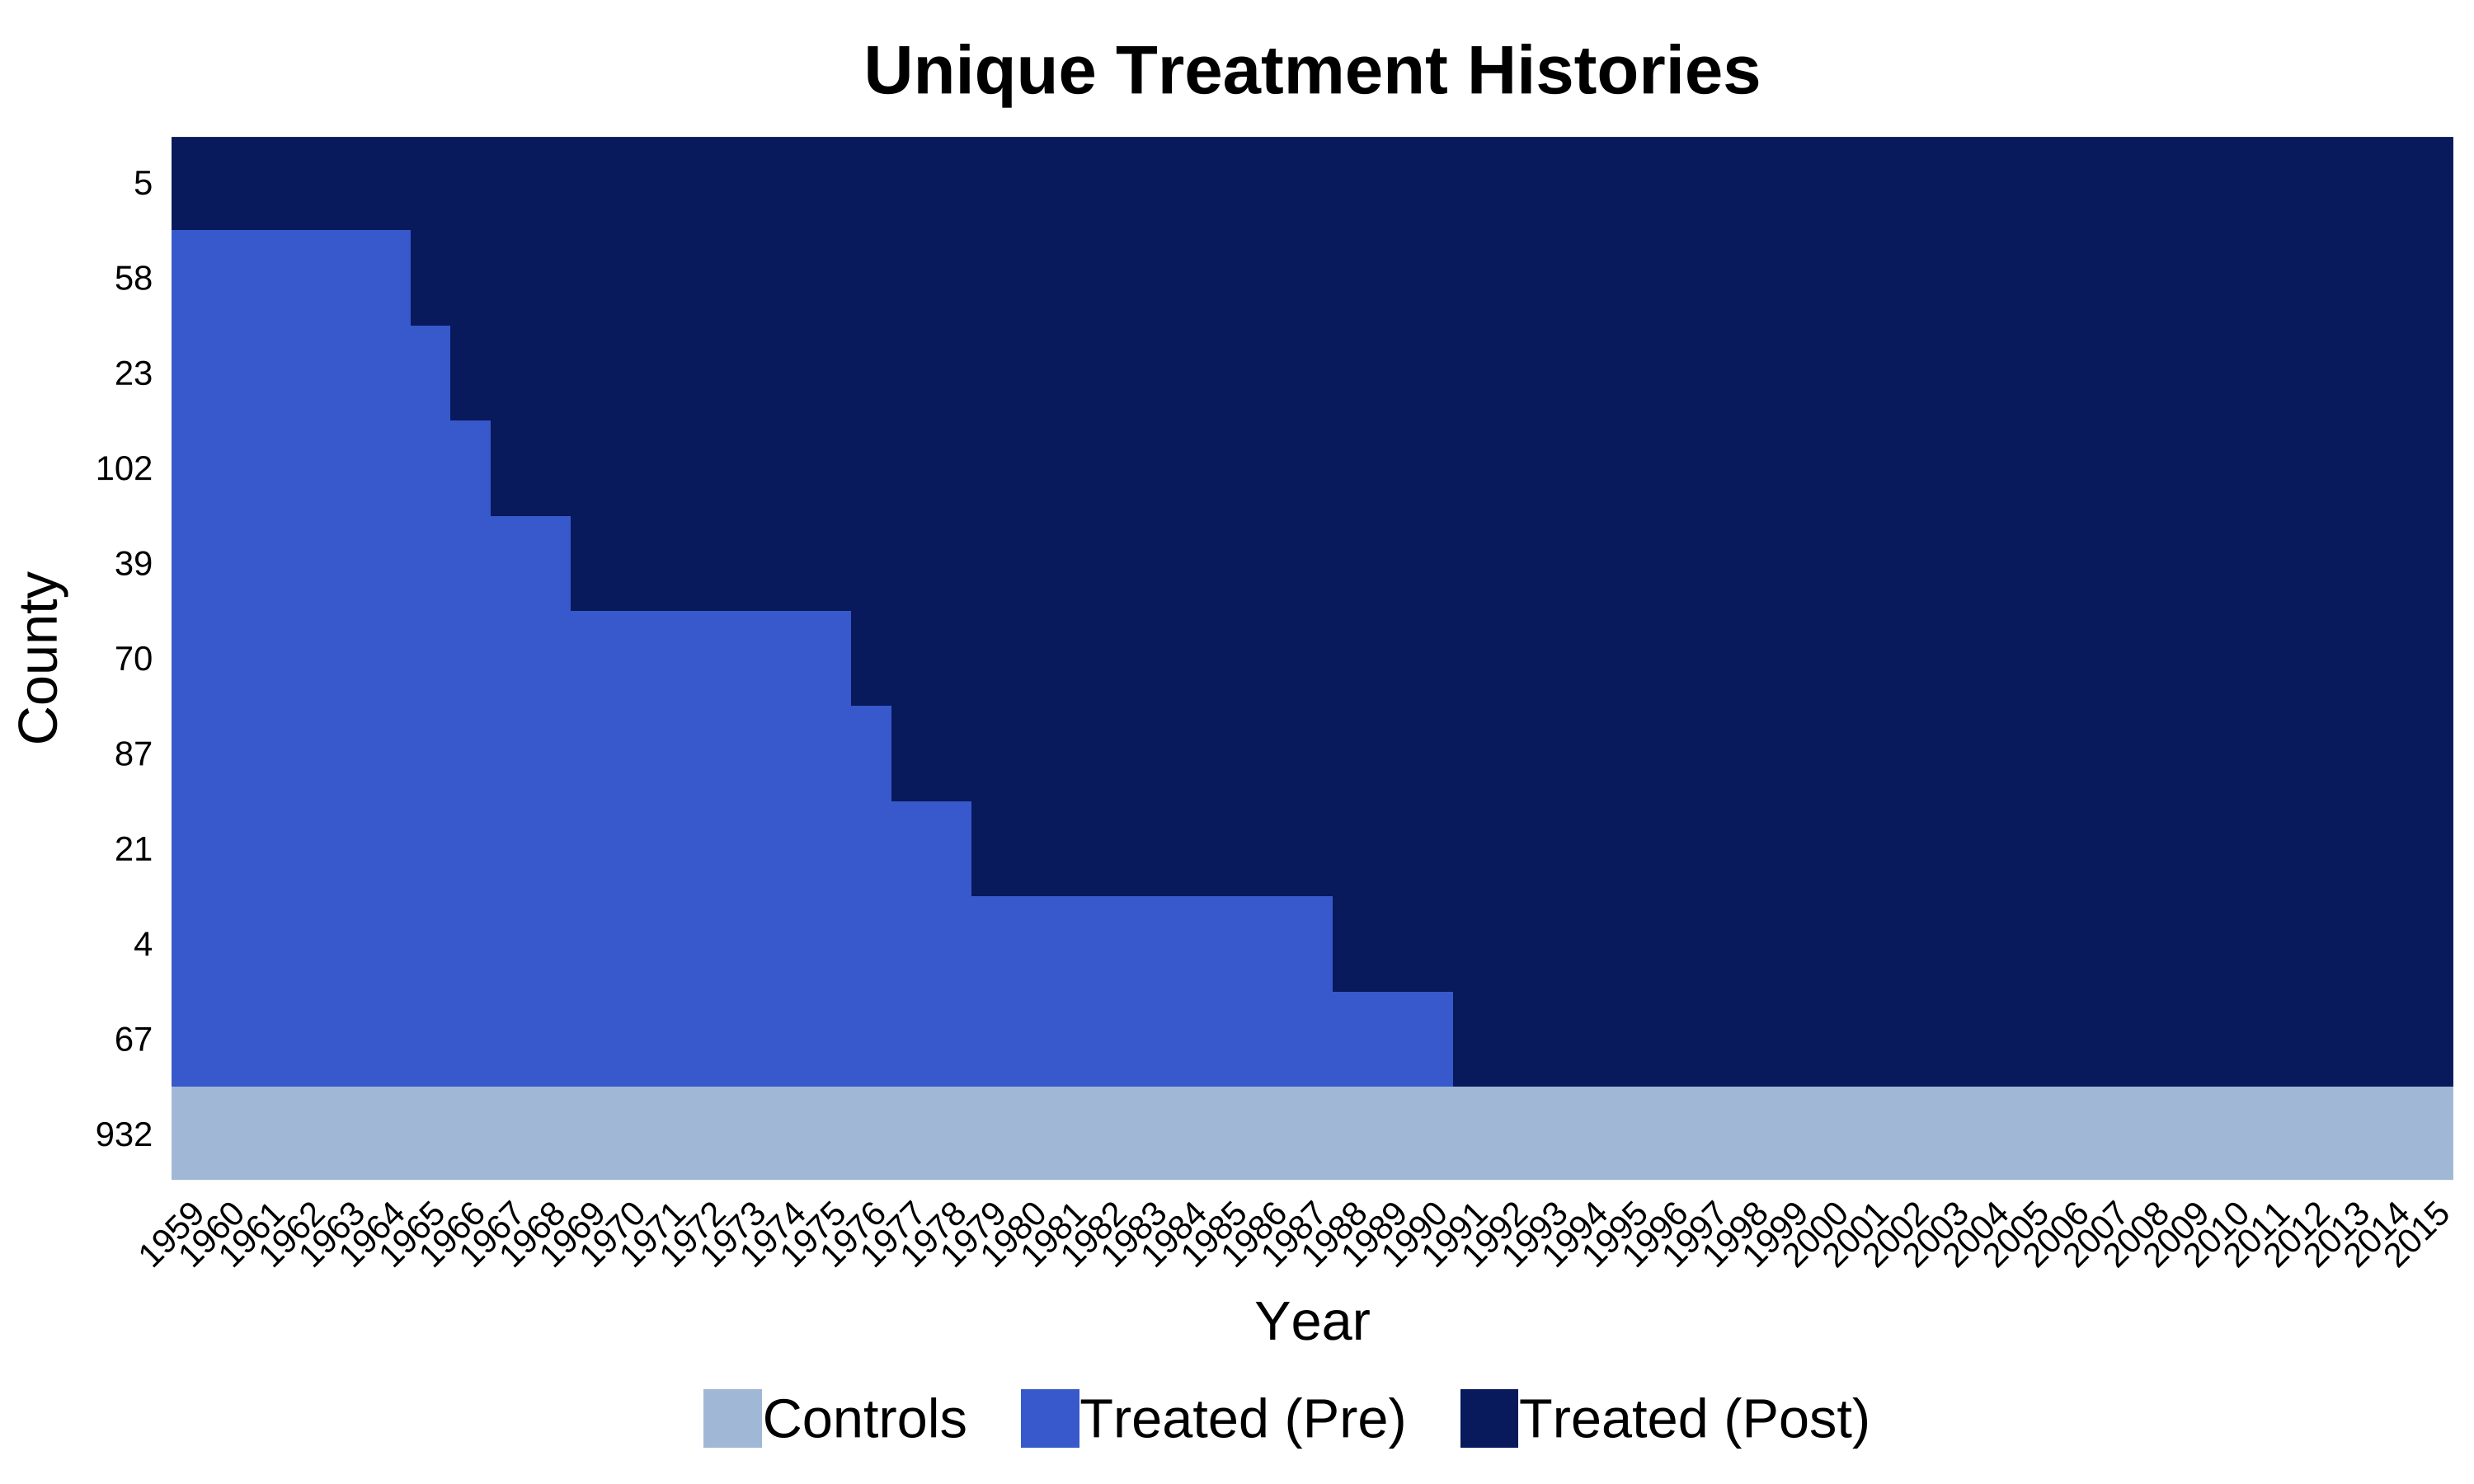
\includegraphics[width=0.8\textwidth]{figures/195-staggarred_sample_panel_view.png}
    \label{fig:194-staggarred_sample_panel_view}

    \begin{minipage}{\linewidth}
    \caption*{\footnotesize{
      \noindent\textit{Note:} This alternative view of policy adoption timing complements Figure~\ref{fig:192-staggarred_sample_panel_view}. It emphasizes the distribution of treated versus control counties over time, helping to validate the use of staggered treatment timing in the empirical strategy.\\
    \noindent\textit{Source:} RAND State Firearm Law Database, 1813–2015.
    }}
  \end{minipage}
\end{figure}

\pagebreak
\clearpage
\begin{figure}[htbp]
    \centering
    \caption{Timing of Waiting Period Policy Adoption Across States That Moved Out of Treatment}
    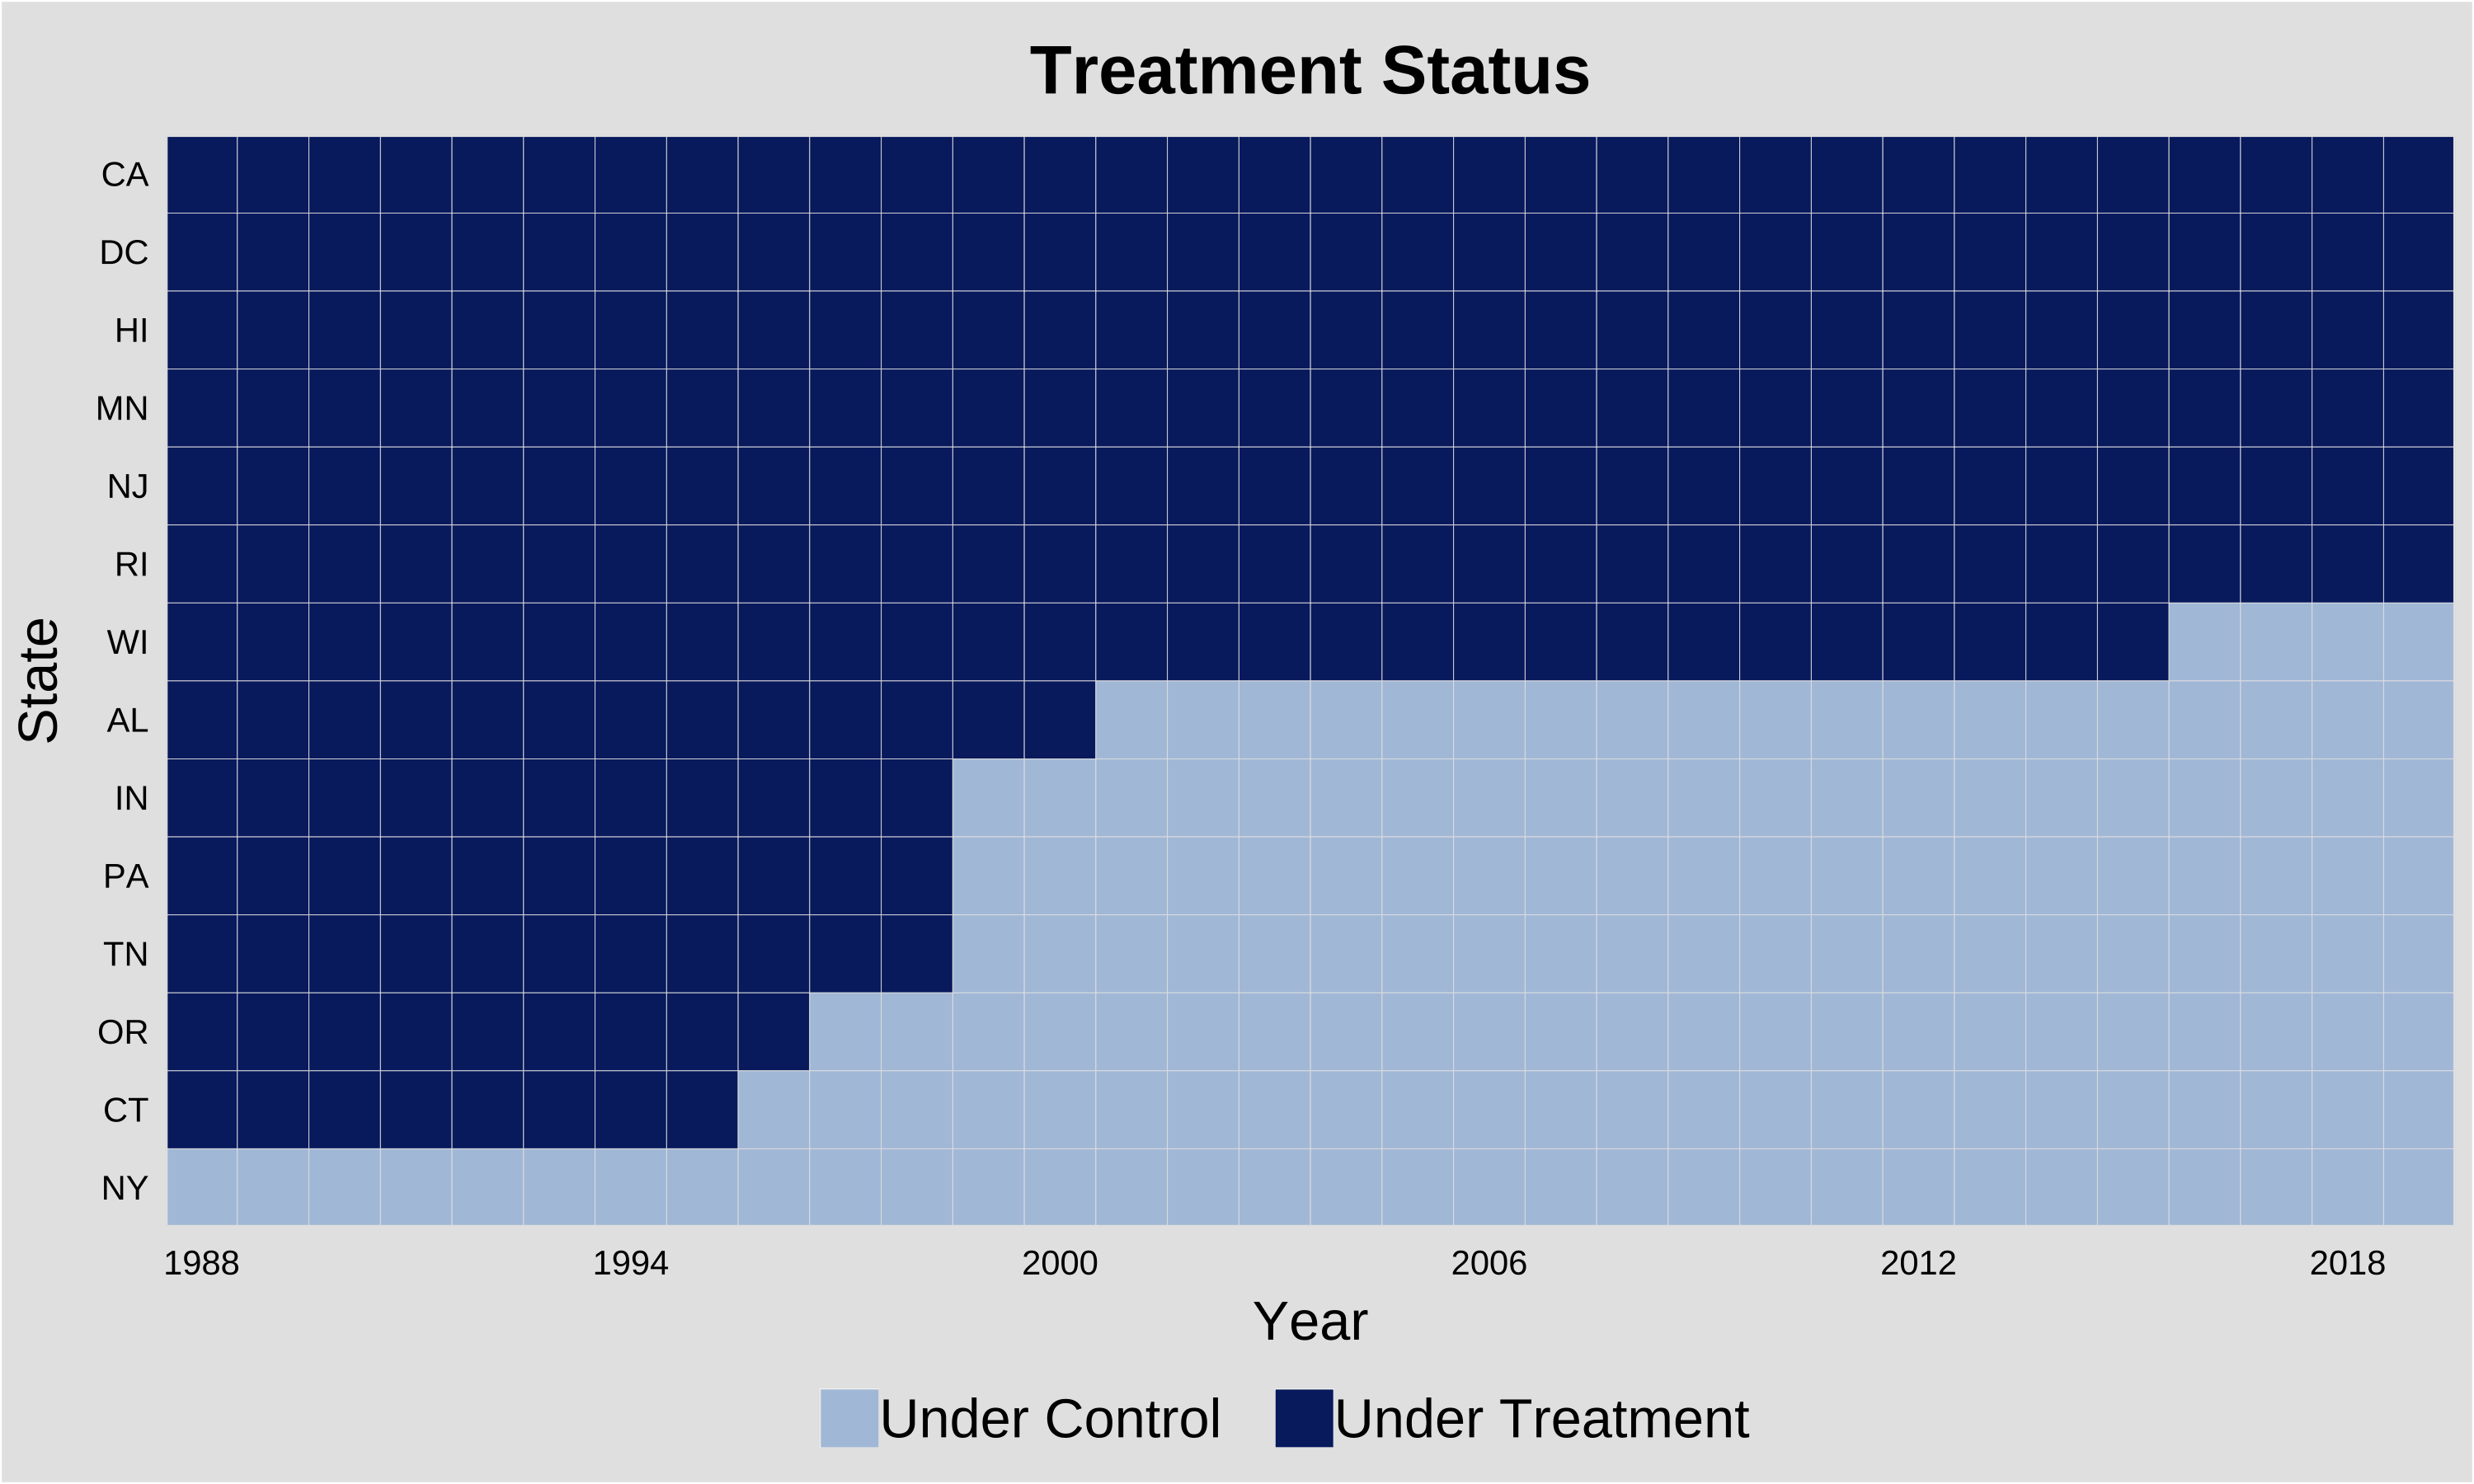
\includegraphics[width=0.8\textwidth]{figures/200-staggarred_sample_out_panel_view.png}
    \label{fig:200-staggarred_sample_out_panel_view}
    \begin{minipage}{\linewidth}
    \caption*{\footnotesize{
      \noindent\textit{Note:} This staggered adoption panel view illustrates the year of waiting period policy implementation for each state included in the study. It provides visual clarity on treatment timing across states, which is crucial for interpreting the event study estimates and understanding the source of identifying variation.\\
    \noindent\textit{Source:} RAND State Firearm Law Database, 1813–2015.
 
    }}
  \end{minipage}
\end{figure}


\pagebreak
\clearpage

\begin{figure}[htbp]
    \centering
    \caption{Timing of Waiting Period Policy Adoption Across States: Number of Counties}    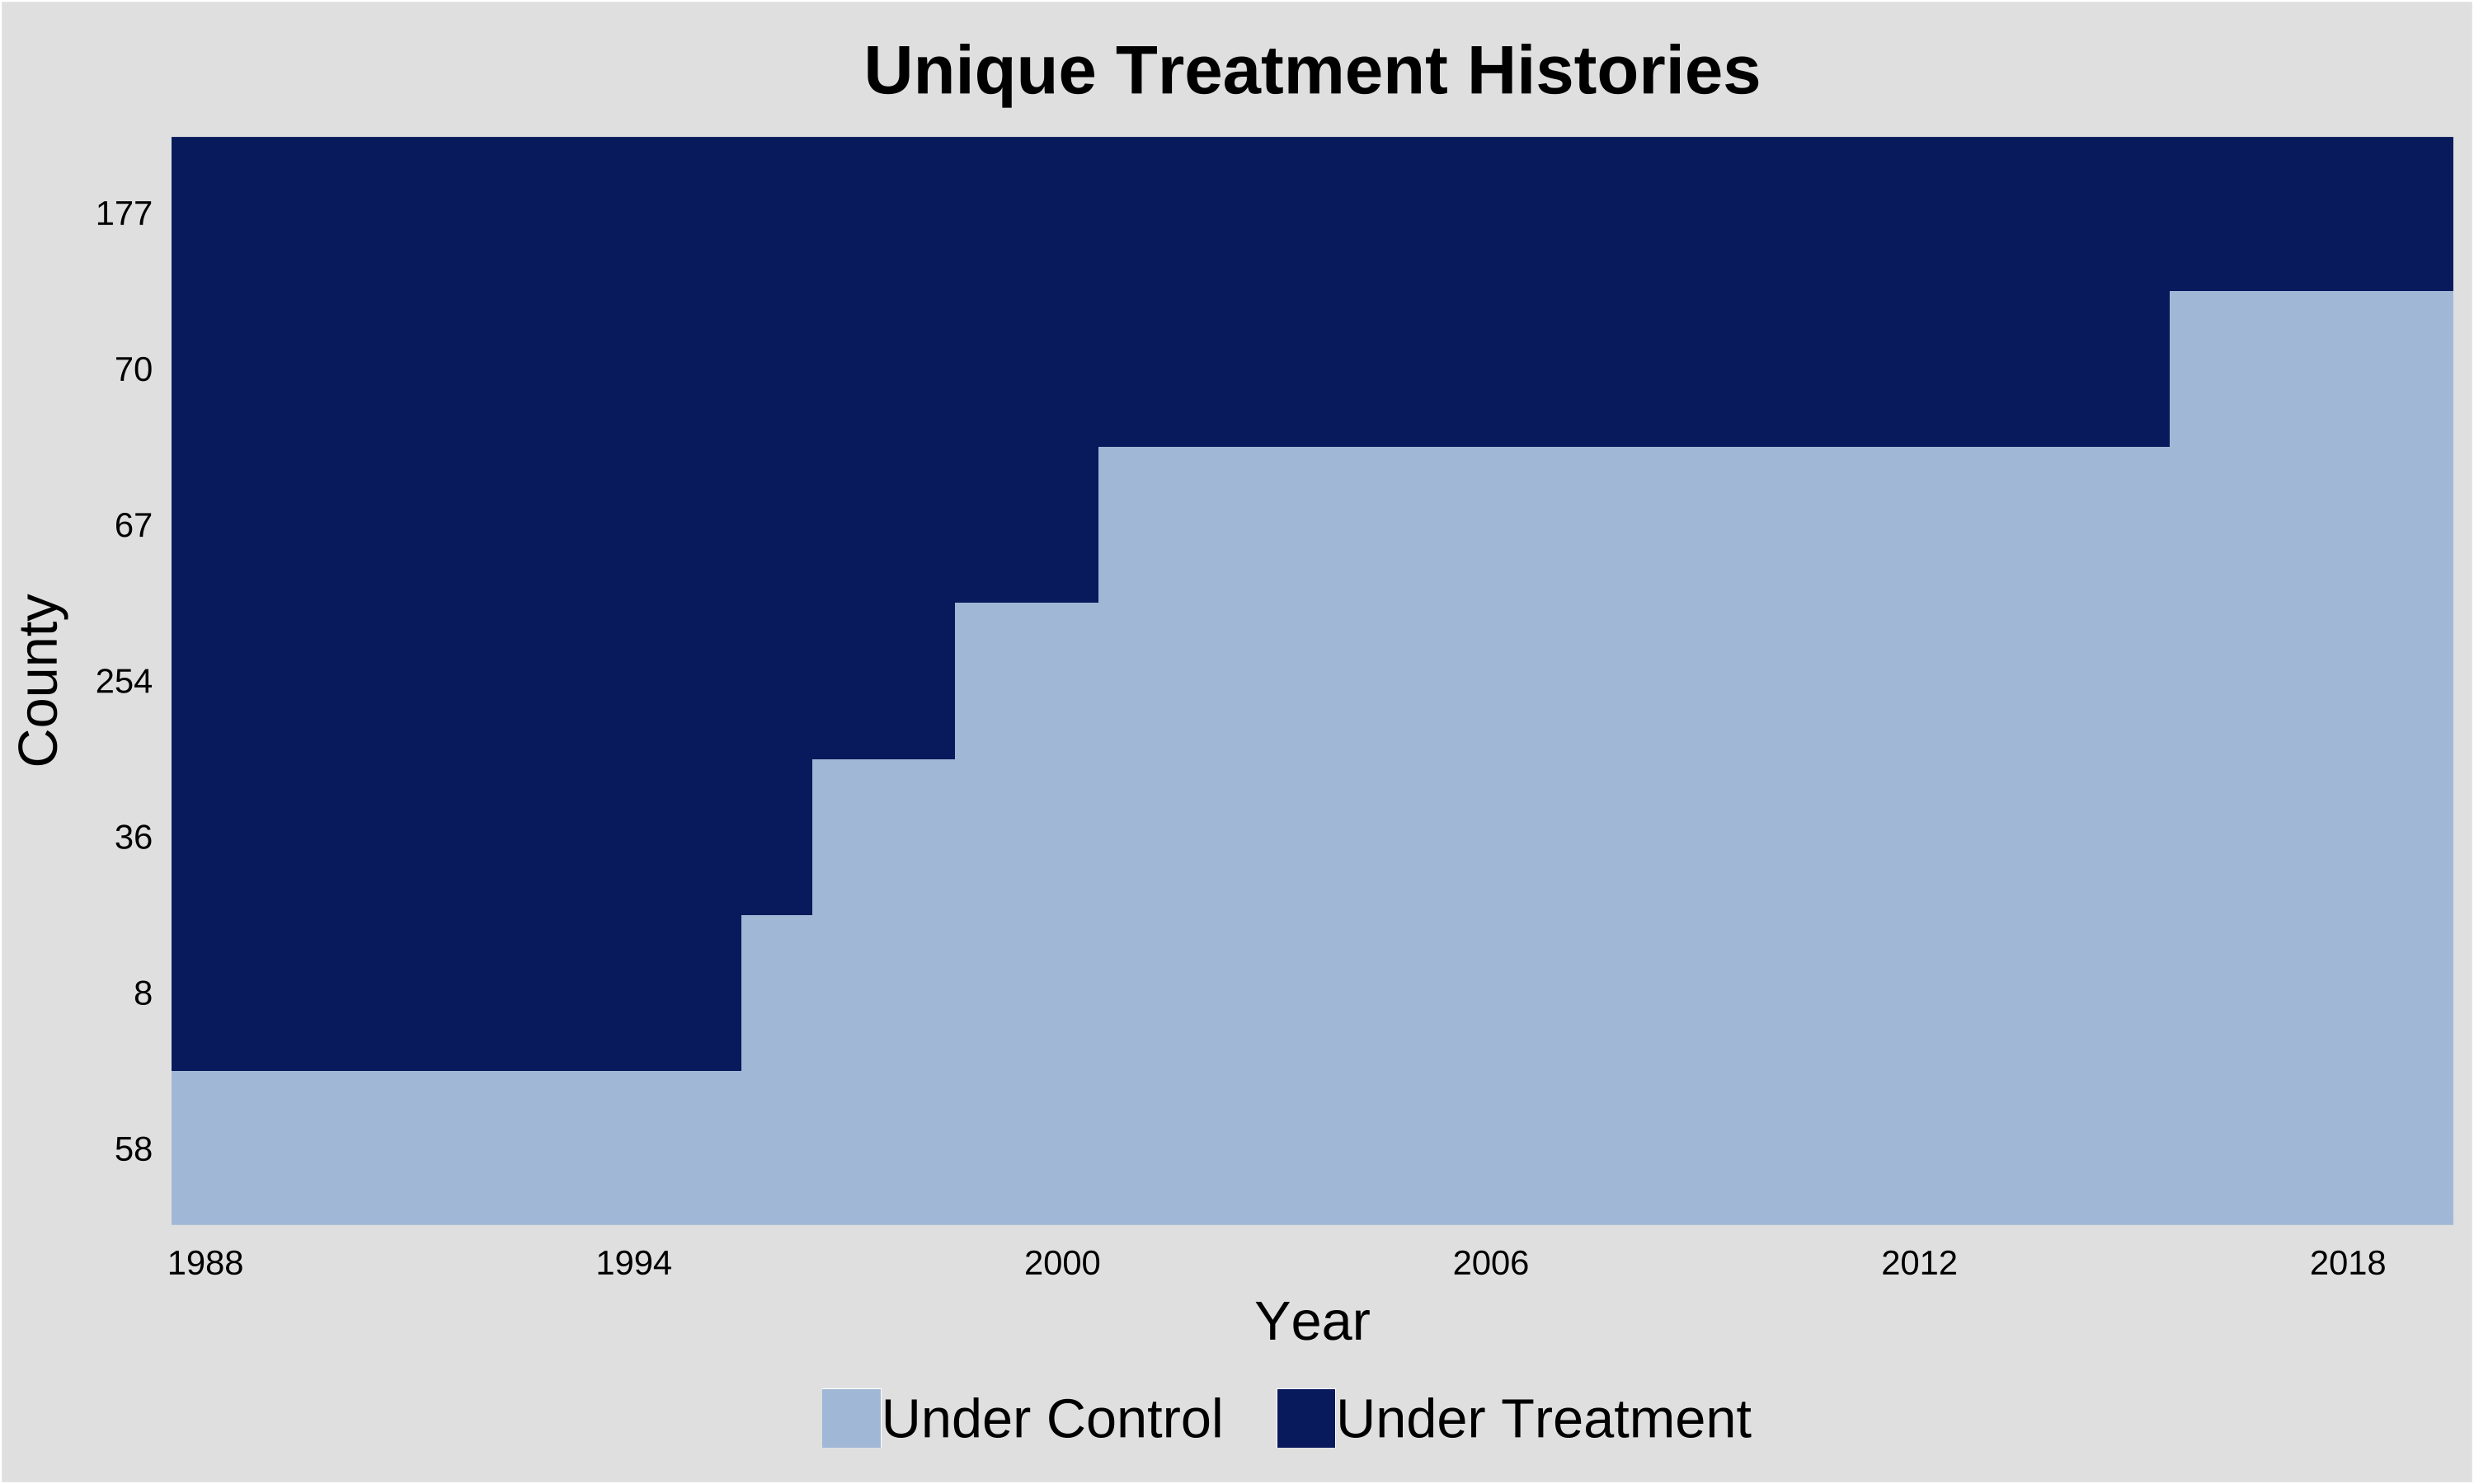
\includegraphics[width=0.8\textwidth]{figures/staggarred_sample_out_panel_view.png}
    \label{fig:staggarred_sample_out_panel_view}

    \begin{minipage}{\linewidth}
    \caption*{\footnotesize{
      \noindent\textit{Note:} This alternative view of policy adoption timing complements Figure~\ref{fig:200-staggarred_sample_out_panel_view}. It emphasizes the distribution of treated versus control counties over time, helping to validate the use of staggered treatment timing in the empirical strategy.\\
    \noindent\textit{Source:} RAND State Firearm Law Database, 1813–2015.
    }}
  \end{minipage}
\end{figure}

\pagebreak
\clearpage

\begin{figure}[htbp]
    \centering
    \caption{Trends in Firearm Suicide Rates Across Counties, 1959–2019}
    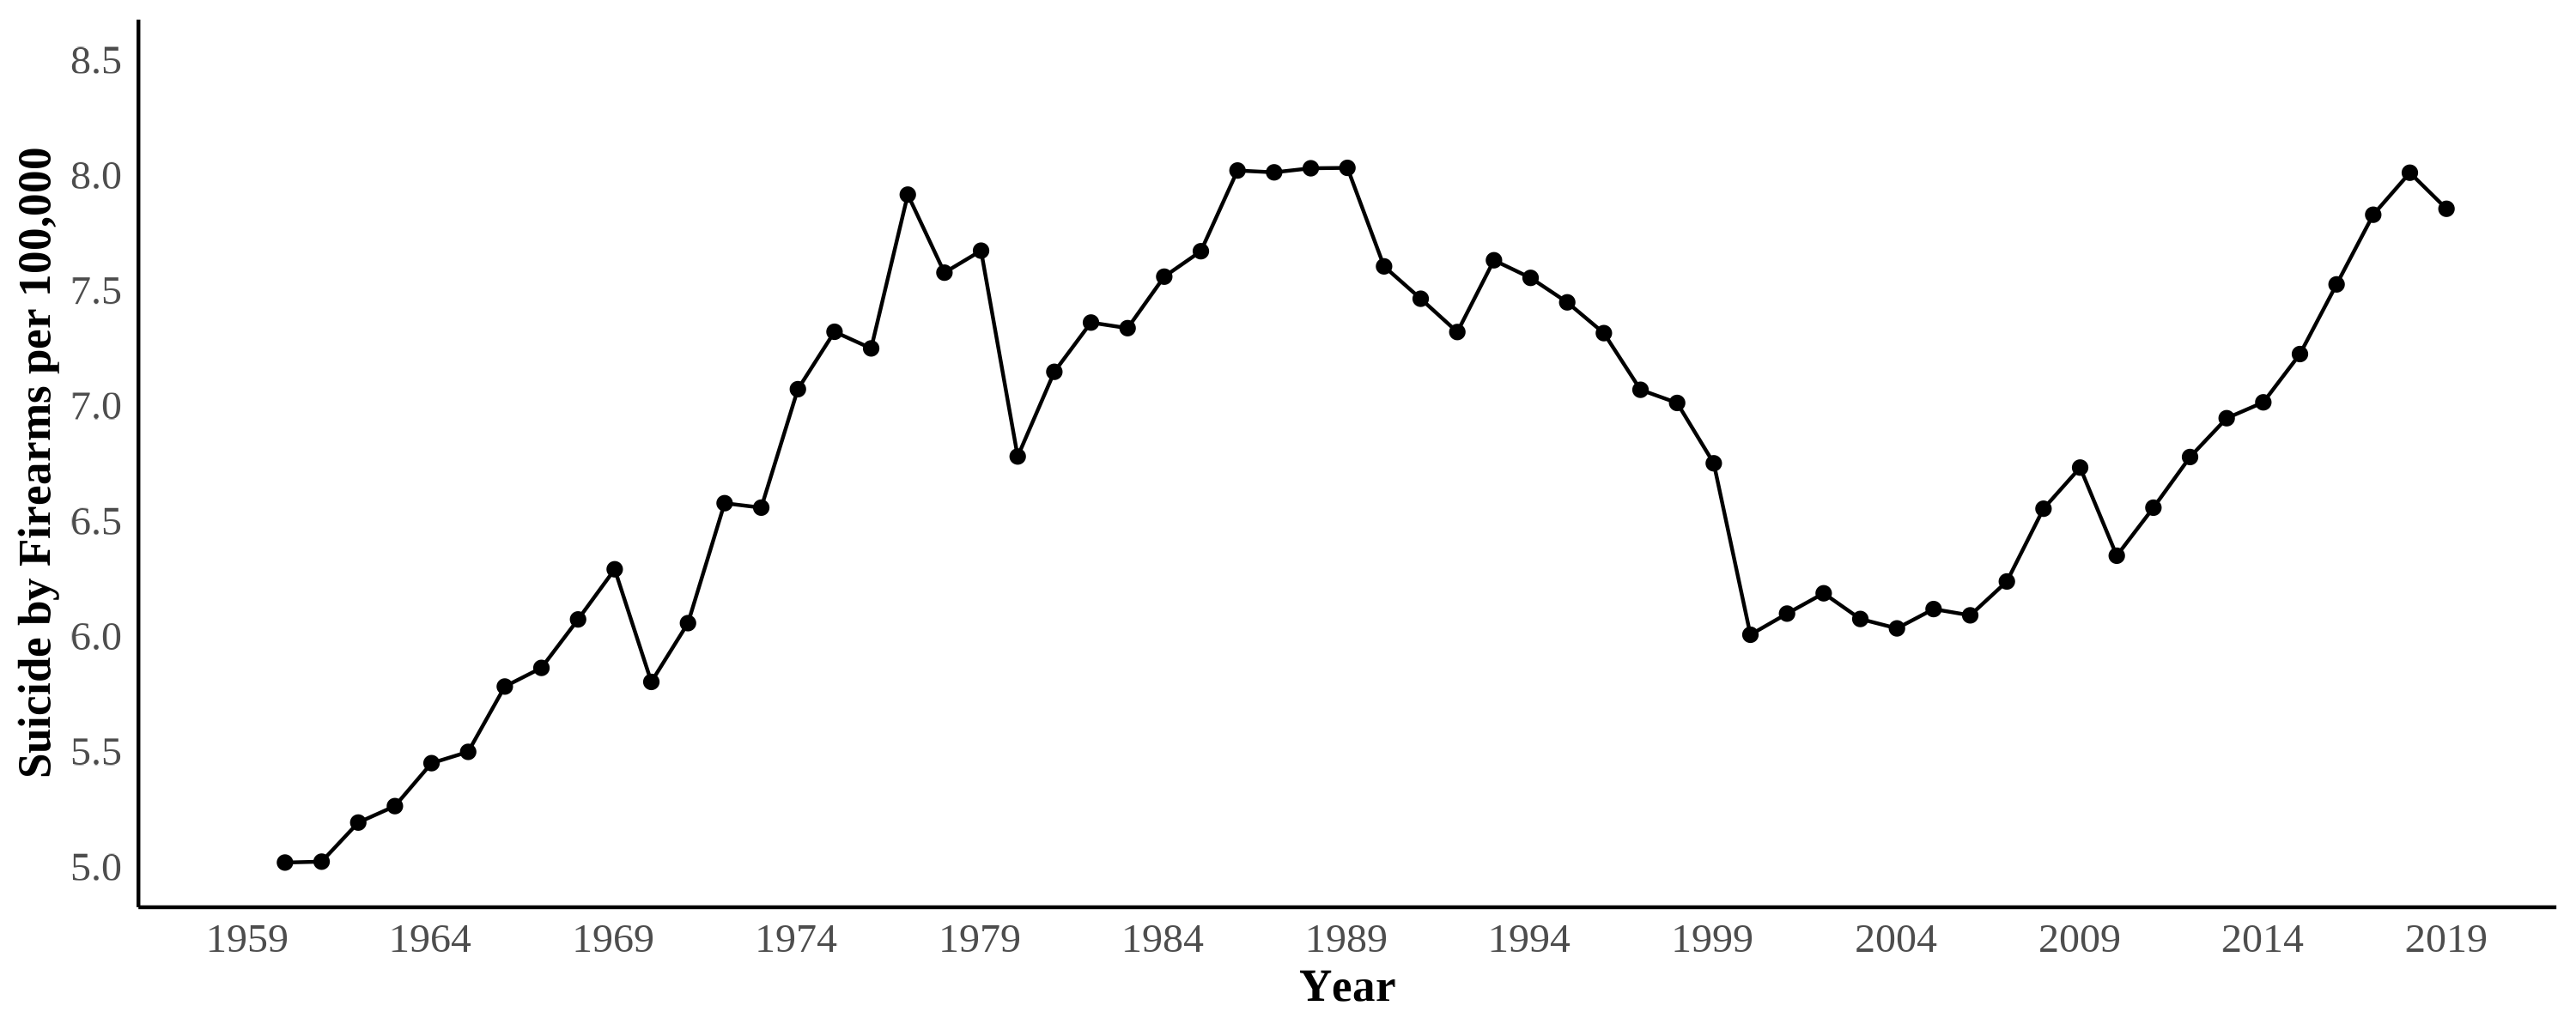
\includegraphics[width=0.8\textwidth]{figures/05-suicide_firearm_byyear_popcont.png}
    \label{fig:suicide_firearm_byyear_popcont}

    \begin{minipage}{\linewidth}
    \caption*{\footnotesize{
      \noindent\textit{Note:} This figure shows the annual trend in suicide rates by firearm (per 100,000 population) across US counties from 1959 to 2019. The figure highlights the long-term trajectory of firearm suicides, providing historical context for analyzing the impact of waiting period laws introduced in different years and states. \\
    \noindent\textit{Source:} National Vital Statistics System (NVSS), Multiple Cause of Death Files, 1959–2019.
    }}
  \end{minipage}
\end{figure}

\pagebreak
\clearpage

\begin{figure}[htbp]
    \centering
    \caption{Trends in Overall Suicide Rates Across Counties, 1959–2019}
    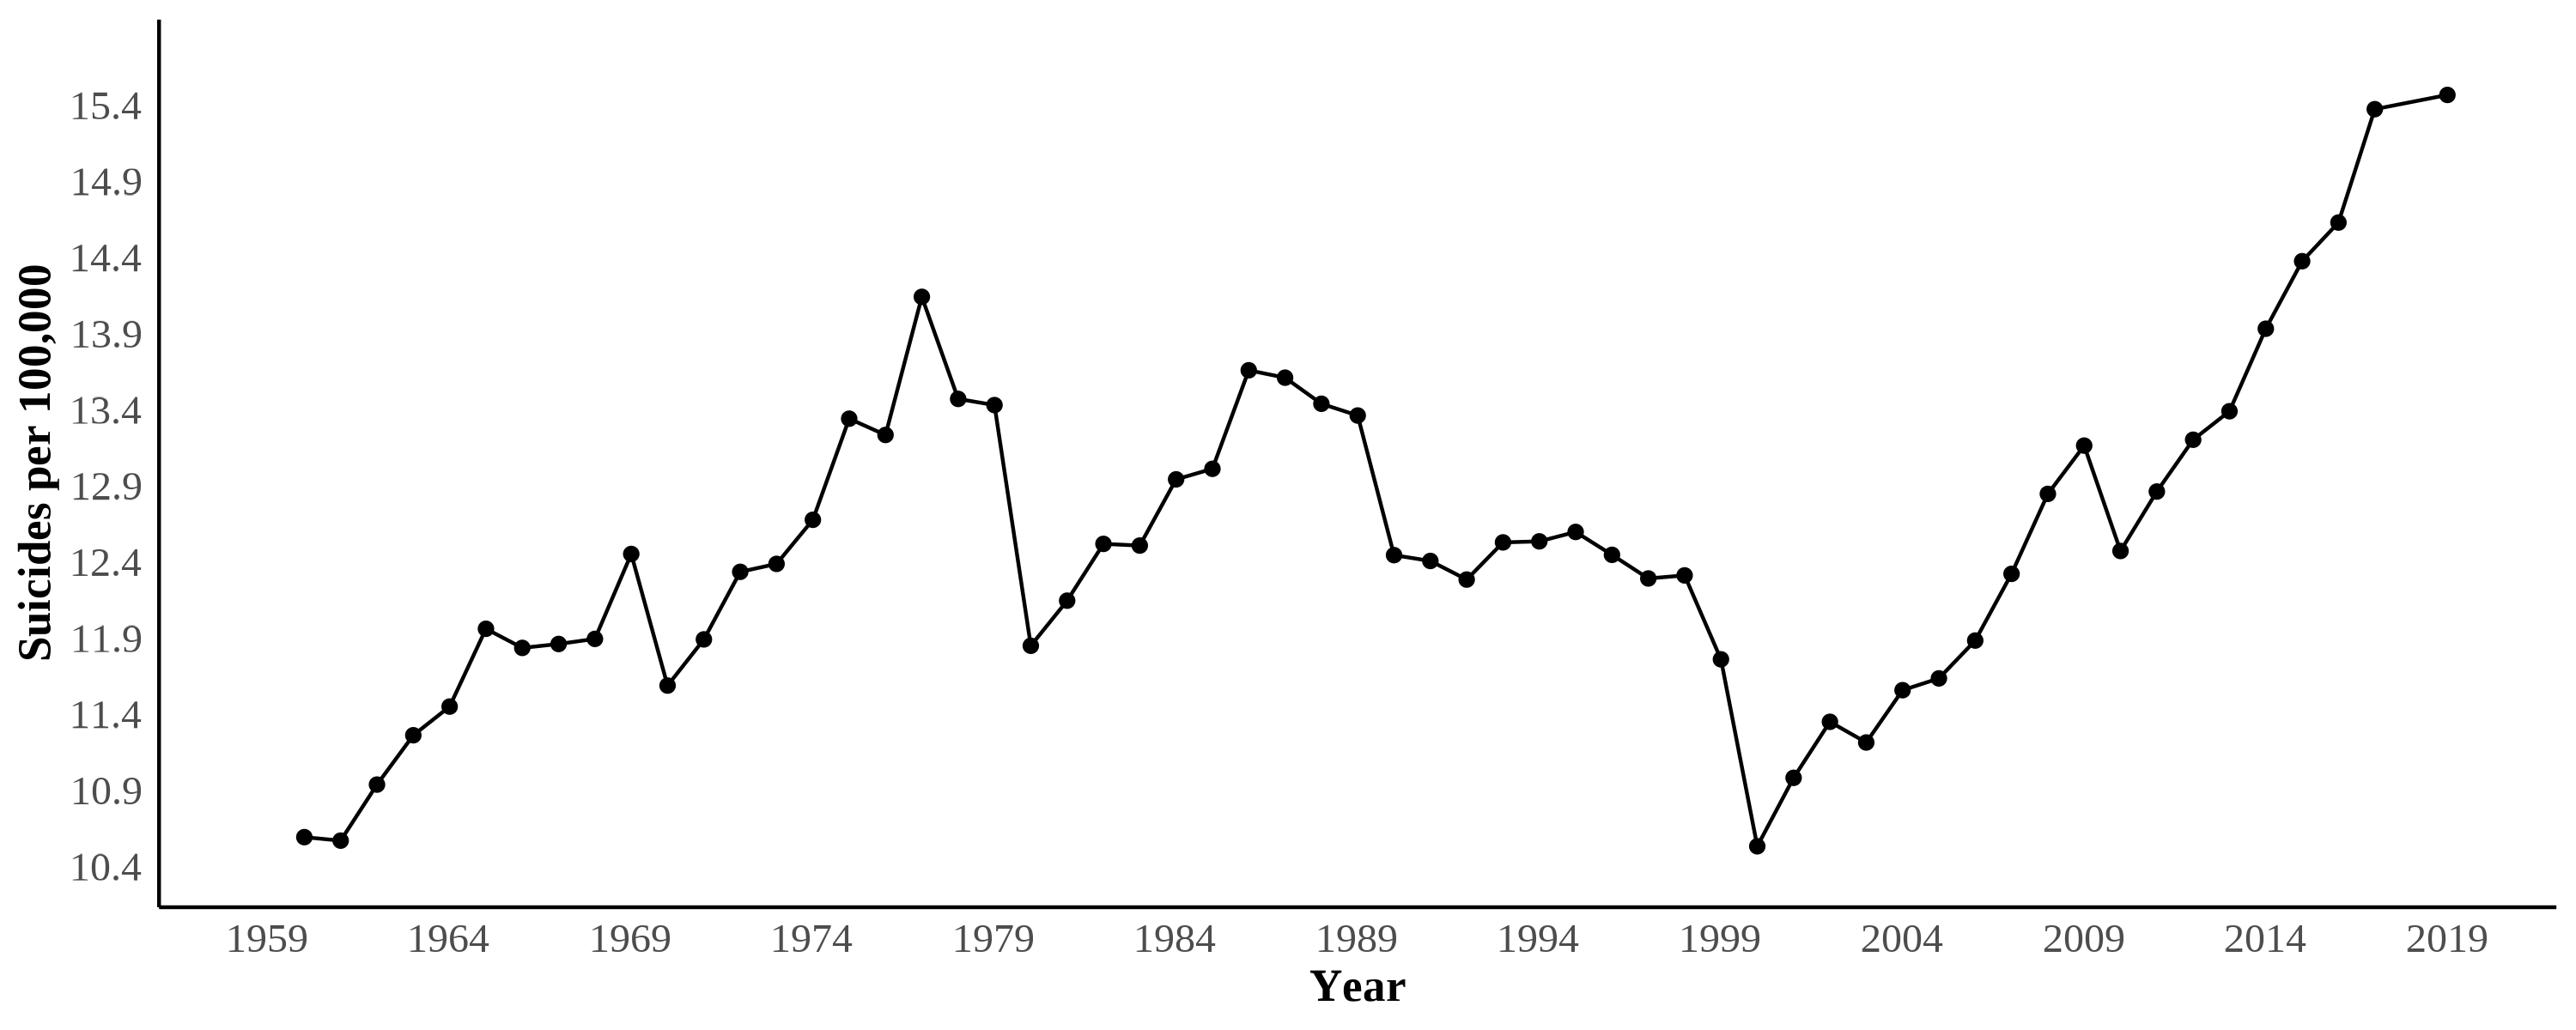
\includegraphics[width=0.8\textwidth]{figures/06-suicide_byyear_popcont.png}
    \label{fig:06-suicide_byyear_popcont}

    \begin{minipage}{\linewidth}
    \caption*{\footnotesize{
      \noindent\textit{Note:} This figure displays the overall suicide rate (all causes, per 100,000 population) from 1959 to 2019. It offers a comparison benchmark for firearm-specific suicides and helps evaluate whether general suicide trends might confound the estimated effects of waiting period policies.\\
    \noindent\textit{Source:} National Vital Statistics System (NVSS), Multiple Cause of Death Files, 1959–2019.
    }}
  \end{minipage}
\end{figure}

\pagebreak
\clearpage

\begin{figure}[htbp]
    \centering
    \caption{Firearm Suicide Rates by State Treatment Status, 1959–2019}
    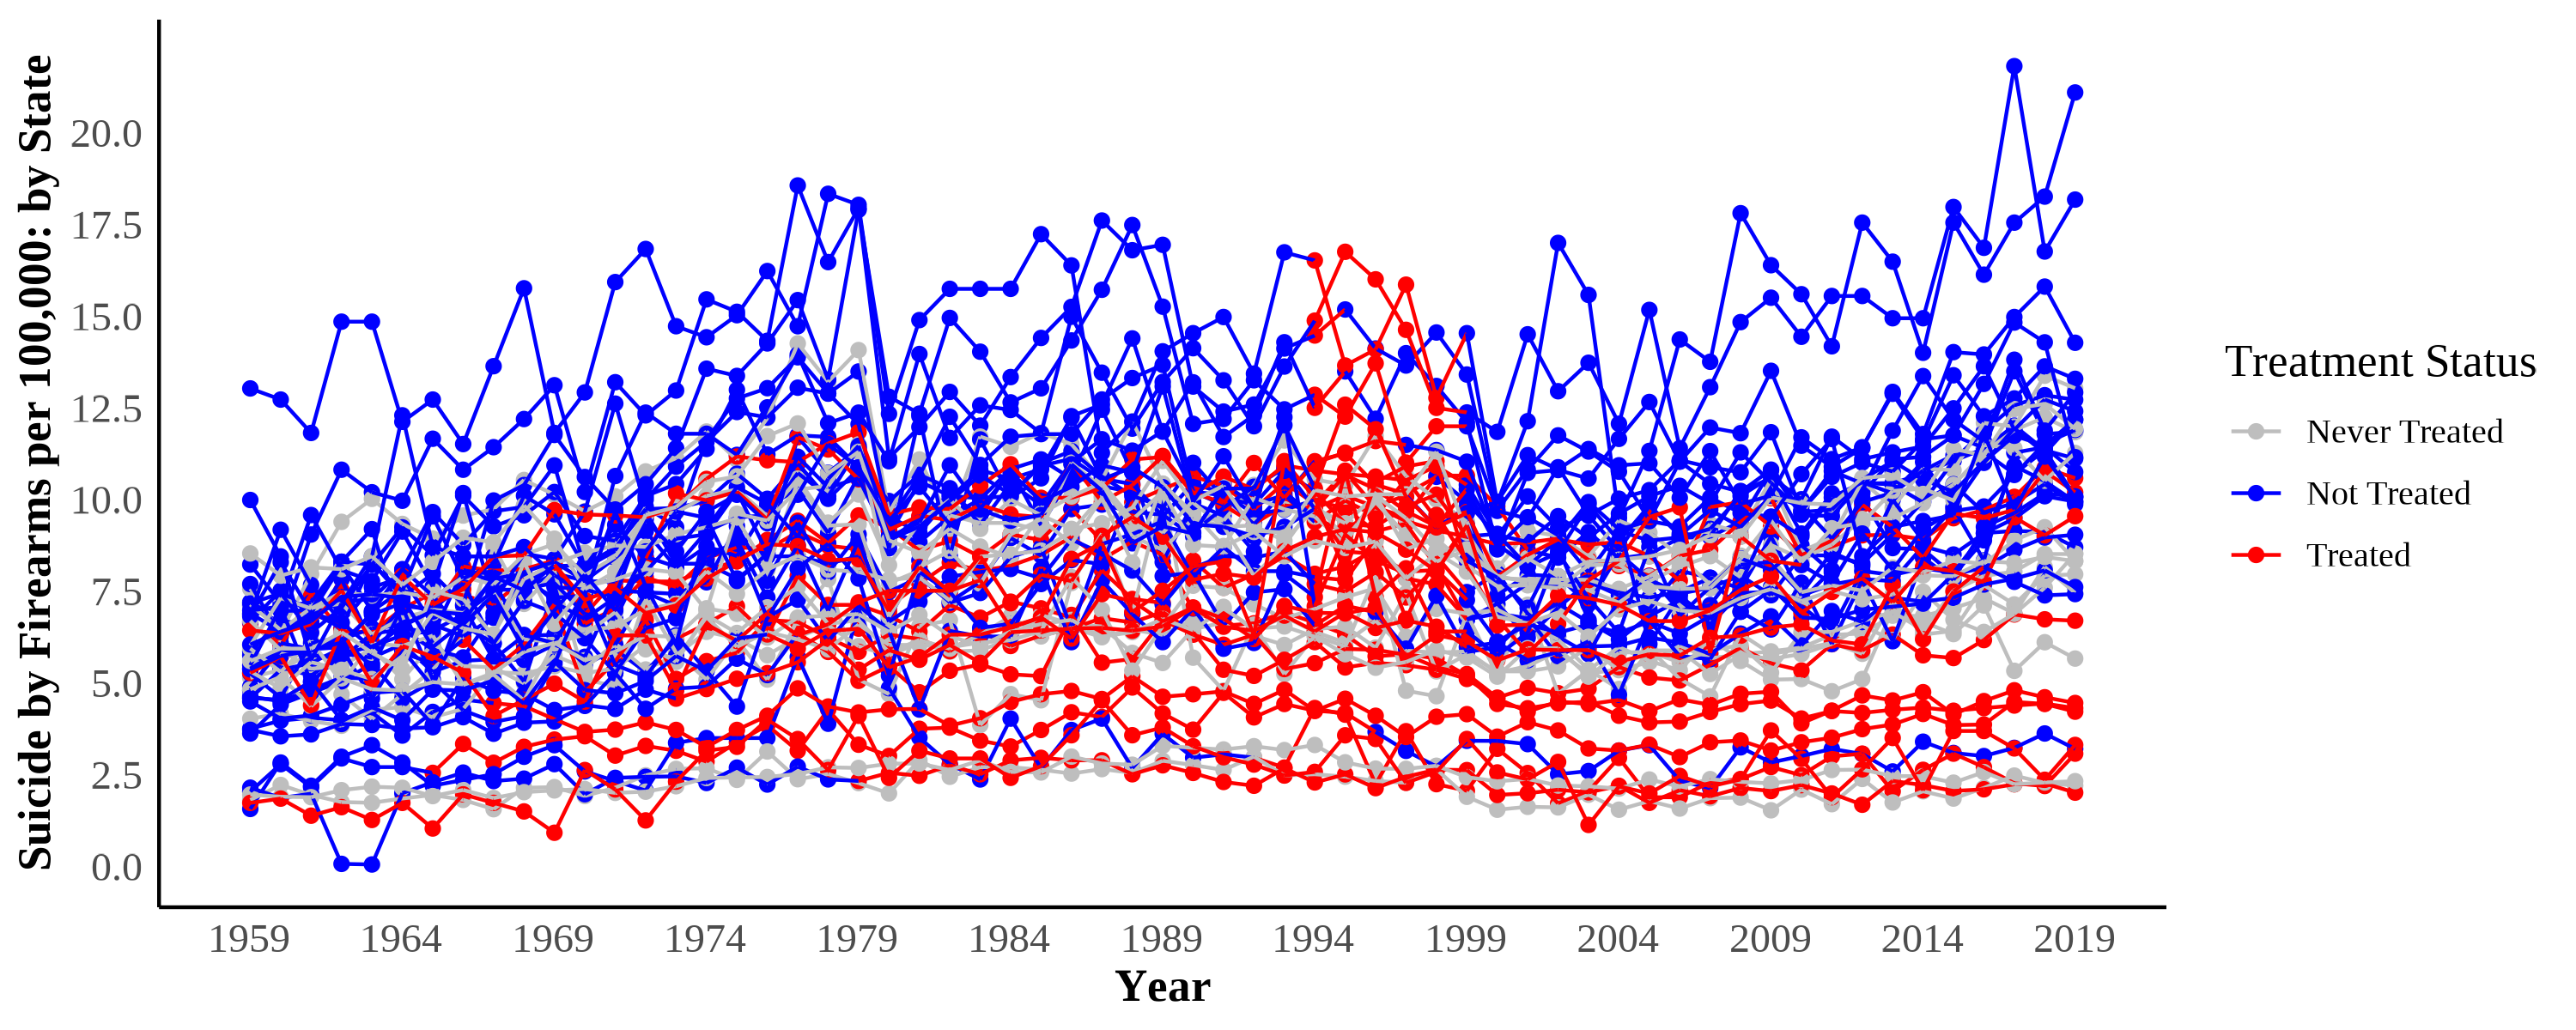
\includegraphics[width=0.8\textwidth]{figures/01-suicide_firearm_byyearbystate.png}
    \label{fig:01-suicide_firearm_byyearbystat}

    \begin{minipage}{\linewidth}
    \caption*{\footnotesize{
      \noindent\textit{Note:} This figure displays firearm suicide rates (per 100,000 population) from 1959 to 2019 across states, categorized by treatment status. "Treated" states implemented waiting period policies, "Not Treated" states never adopted such policies during the study period, and "Never Treated" states represent the control group. The consistently lower rates in treated states suggest a potential protective effect of waiting period legislation on firearm suicide mortality. \\
    \noindent\textit{Source:} National Vital Statistics System (NVSS), Multiple Cause of Death Files, 1959–2019.
    }}
  \end{minipage}
\end{figure}

\pagebreak
\clearpage

\begin{figure}[htbp]
    \centering
    \caption{Firearm Suicide Rates by Demographic Group in the US, 1959–2019}
    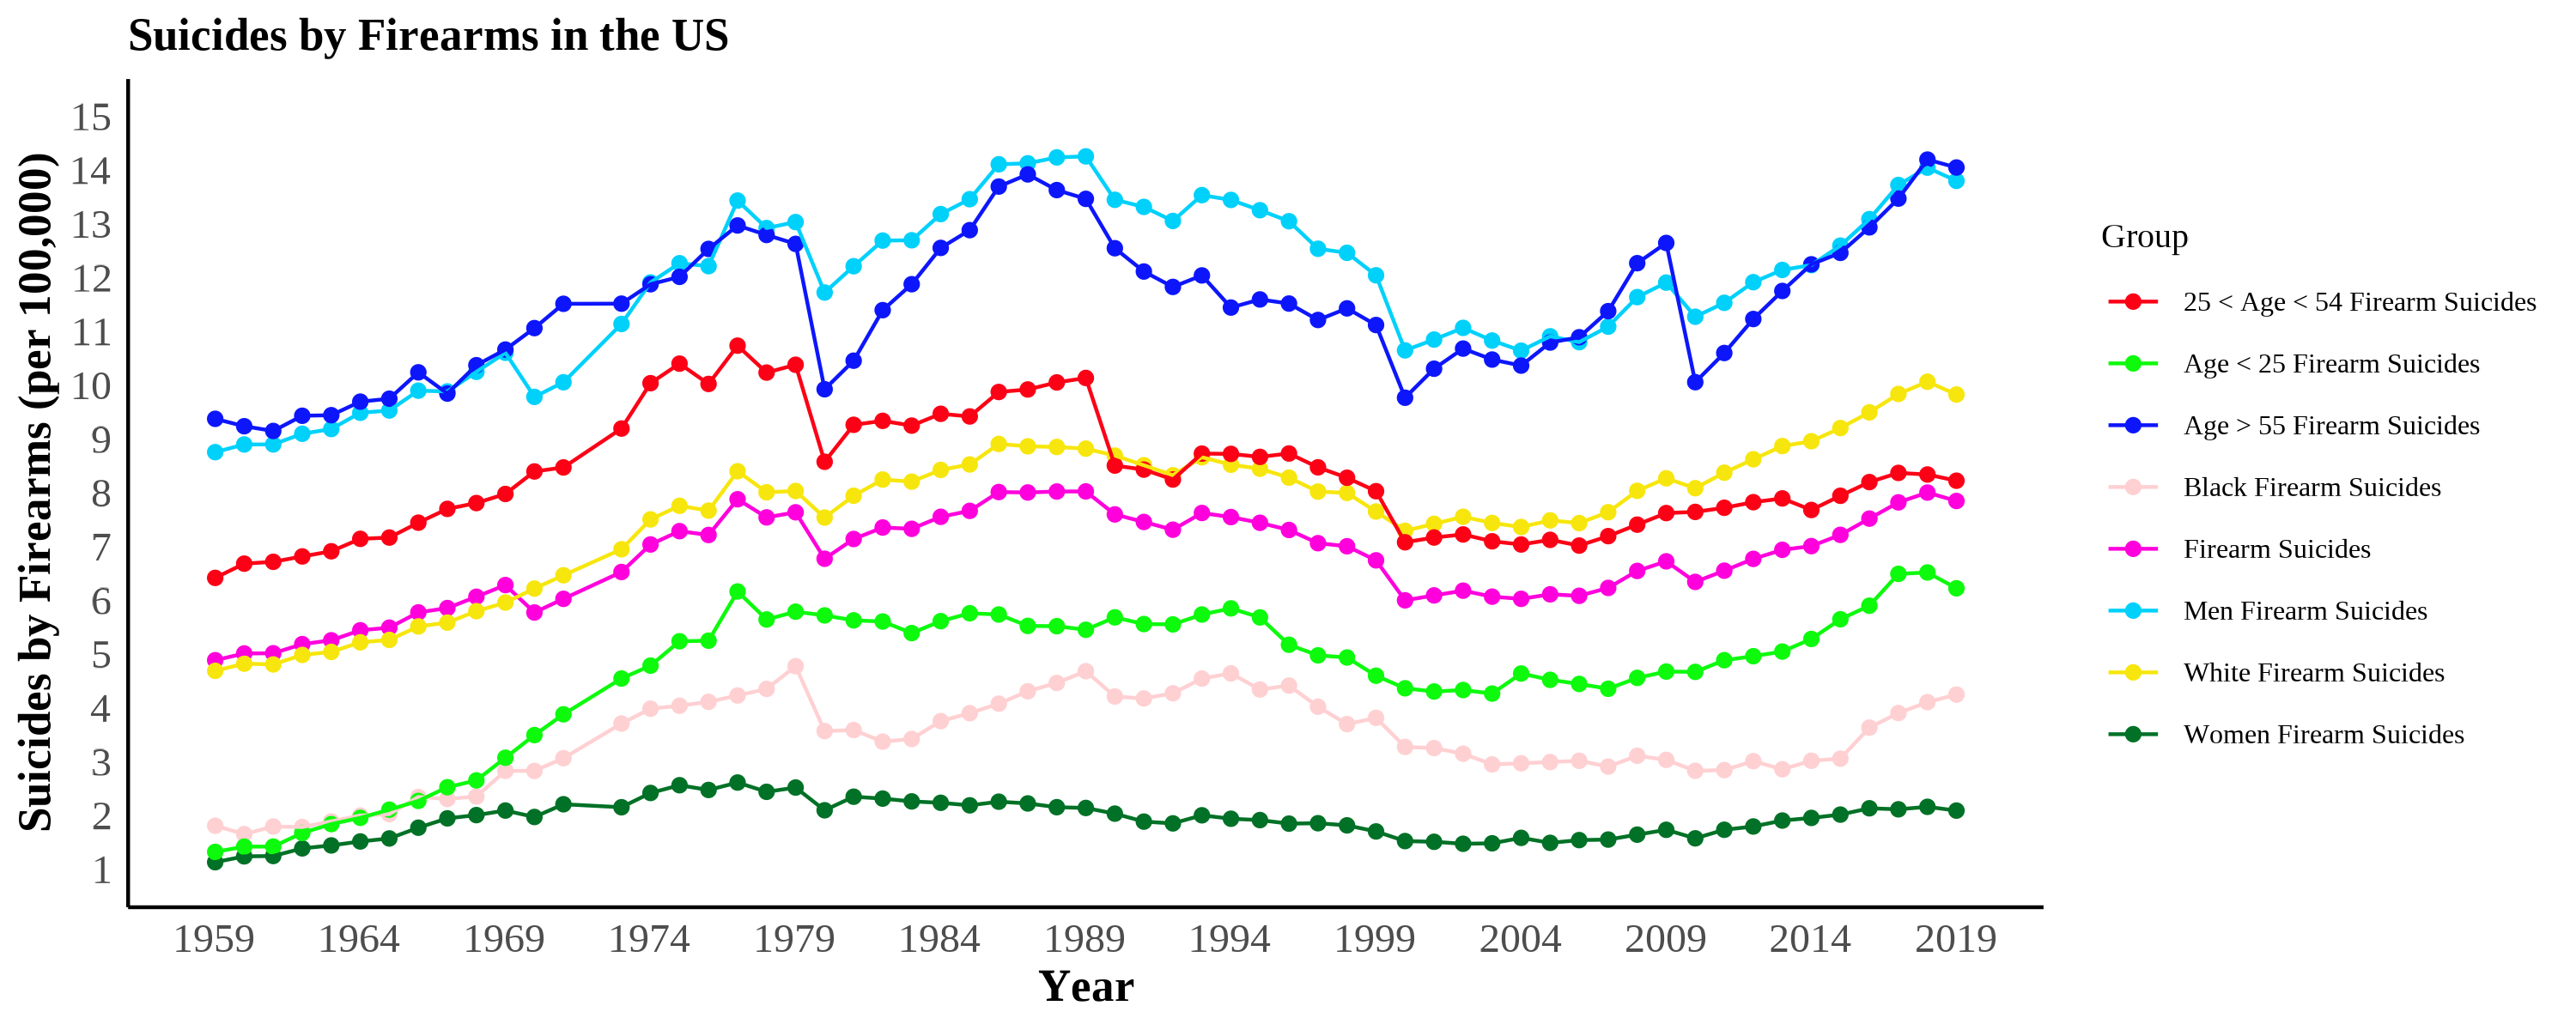
\includegraphics[width=0.8\textwidth]{figures/221-suicide_firearm_byyear_raceagesex.png}
    \label{fig:221-suicide_firearm_byyear_raceagesex}

    \begin{minipage}{\linewidth}
    \caption*{\footnotesize{
      \noindent\textit{Note:} This figure illustrates firearm suicide rates (per 100,000 population) across demographic categories from 1959 to 2019. The substantial differences between men and women, age groups, and racial categories highlight the importance of demographic-specific approaches to suicide prevention. The recent increases across multiple groups after 2010 suggest concerning trends that may warrant targeted intervention strategies.\\
    \noindent\textit{Source:} National Vital Statistics System (NVSS), Multiple Cause of Death Files, 1959–2019.
    }}
  \end{minipage}
\end{figure}
\pagebreak
\clearpage

\begin{figure}[htbp]
    \centering
    \caption{Estimated Effect of Waiting Periods on Overall Firearm Suicide Rates}
    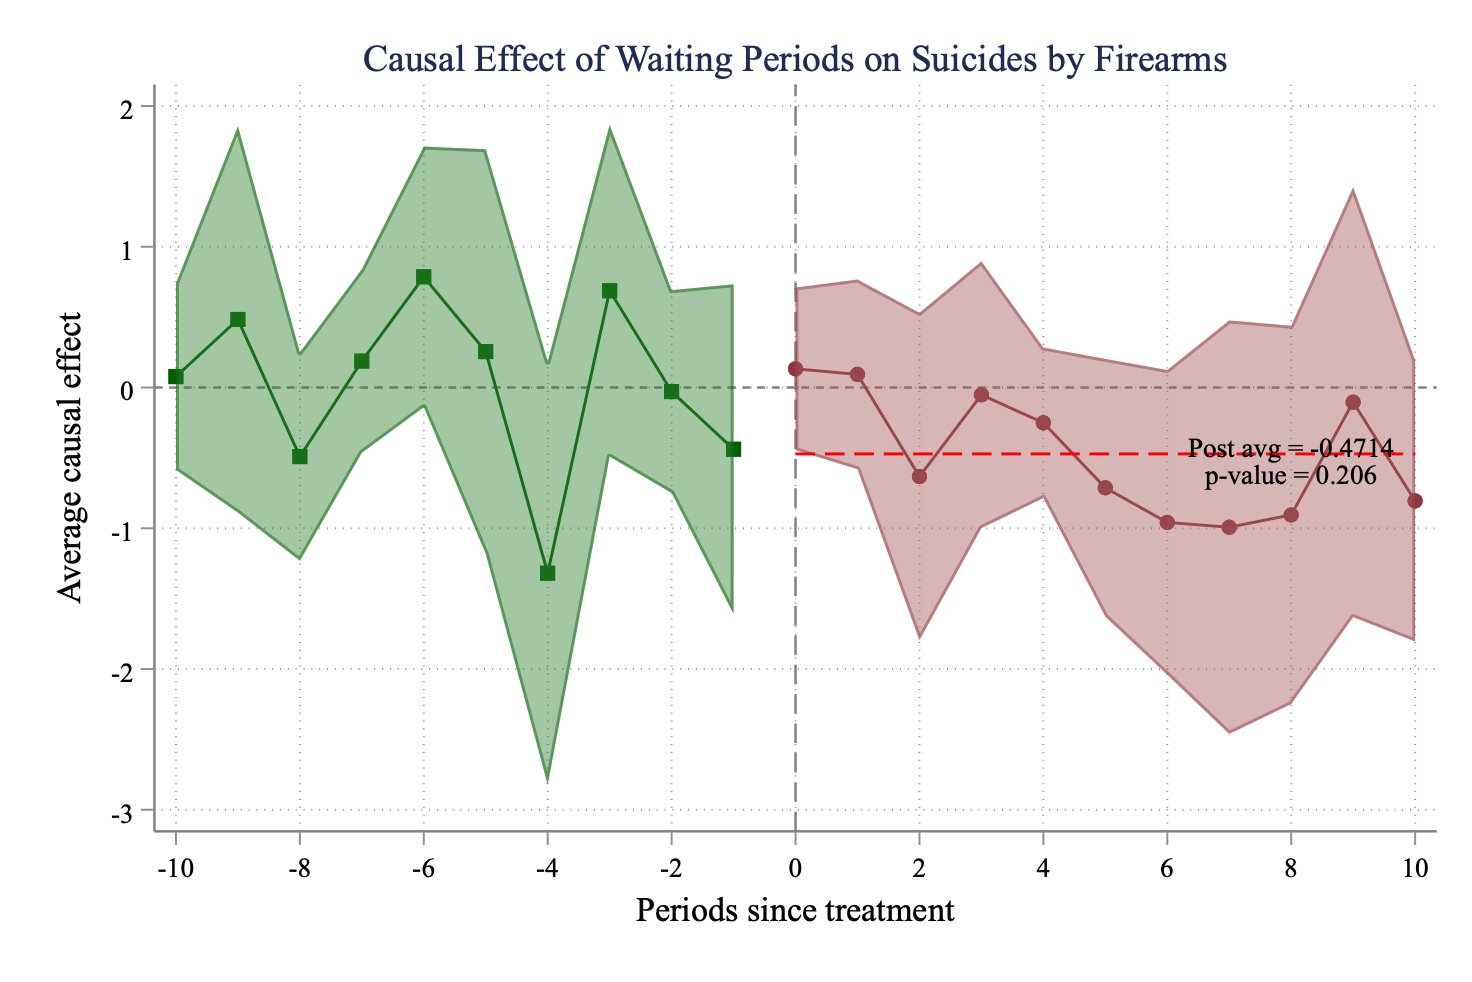
\includegraphics[width=0.8\textwidth]{figures/1035-csid-all-fire-noNY.png}
    \label{fig:firearm_suicide_DID_overall}

    \begin{minipage}{\linewidth}
    \caption*{\footnotesize{
      \noindent\textit{Note:} This figure shows the dynamic effects of waiting period laws on firearm suicide rates across US counties. Each point represents the estimated difference in firearm suicide rates relative to the year of policy adoption (year 0), with 95\% confidence intervals. Standard errors are bootstrapped and clustered at the state level.

 
    }}
  \end{minipage}
\end{figure}

\pagebreak
\clearpage

\begin{figure}[htbp]
    \centering
    \caption{Effect of Waiting Periods on Firearm Suicide Rates Among Men}
    \label{fig:firearm_suicide_DID_men}
    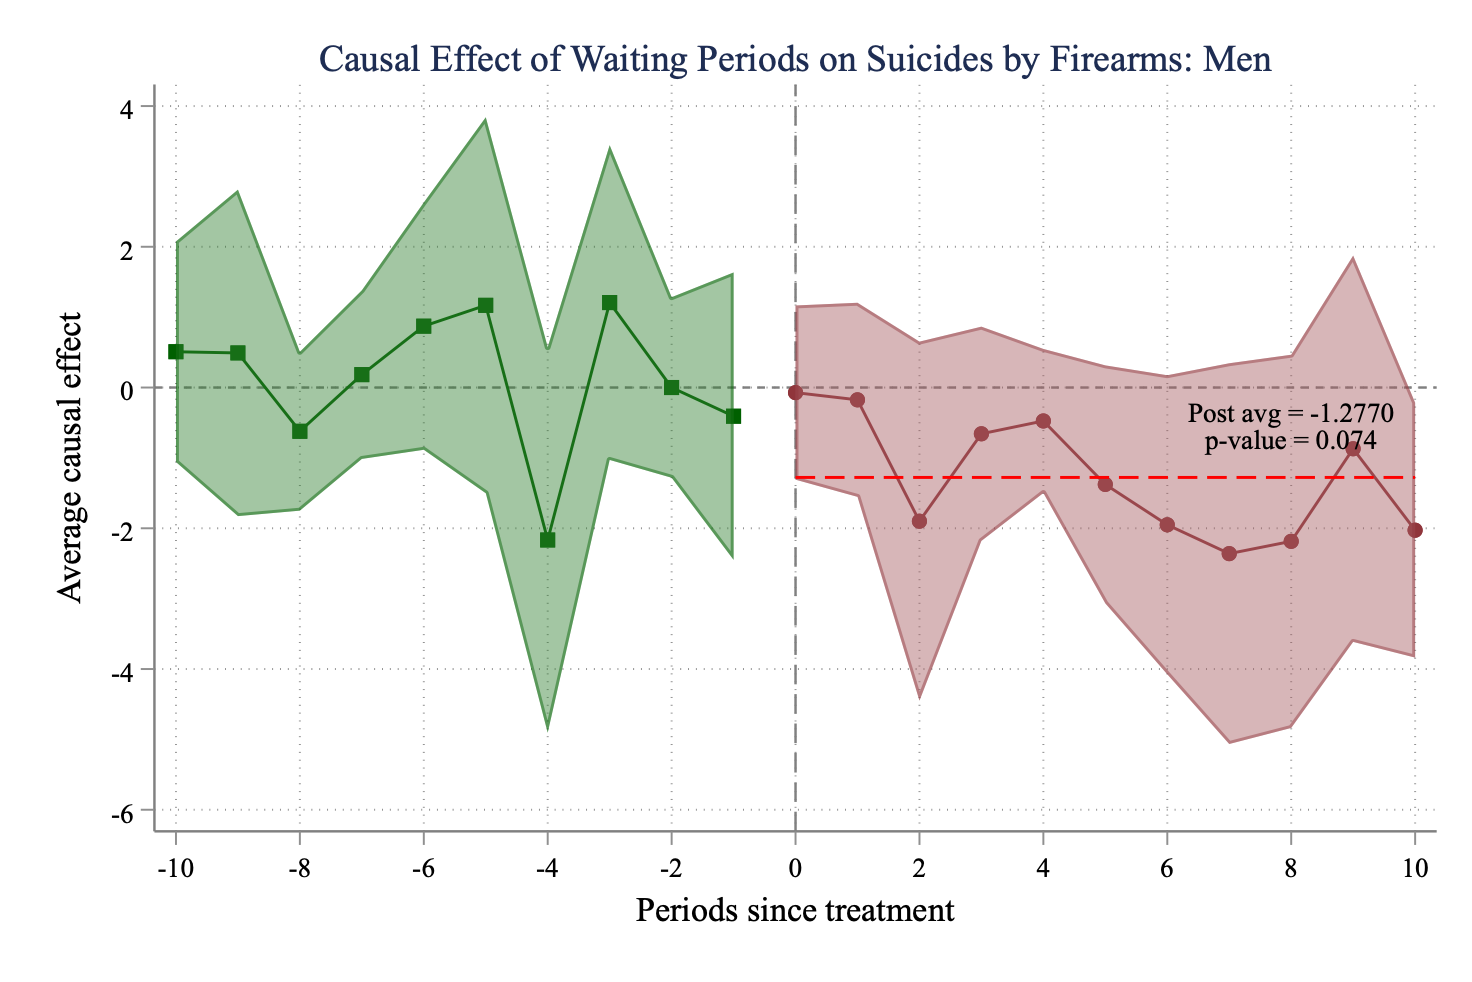
\includegraphics[width=0.8\textwidth]{figures/1036-csid-men-fire-noNY.png}
    \begin{minipage}{\linewidth}
    \caption*{\footnotesize{
      \noindent\textit{Note:} This figure focuses on the male population, showing how waiting period laws affect firearm suicide rates for men specifically. Standard errors are bootstrapped and clustered at the state level. 
    }}
  \end{minipage}
\end{figure}

\pagebreak
\clearpage

\begin{figure}[htbp]
    \centering
    \caption{Effect of Waiting Periods on Firearm Suicide Rates Among Adults Aged 55+}
    \label{fig:firearm_suicide_DID_older}
    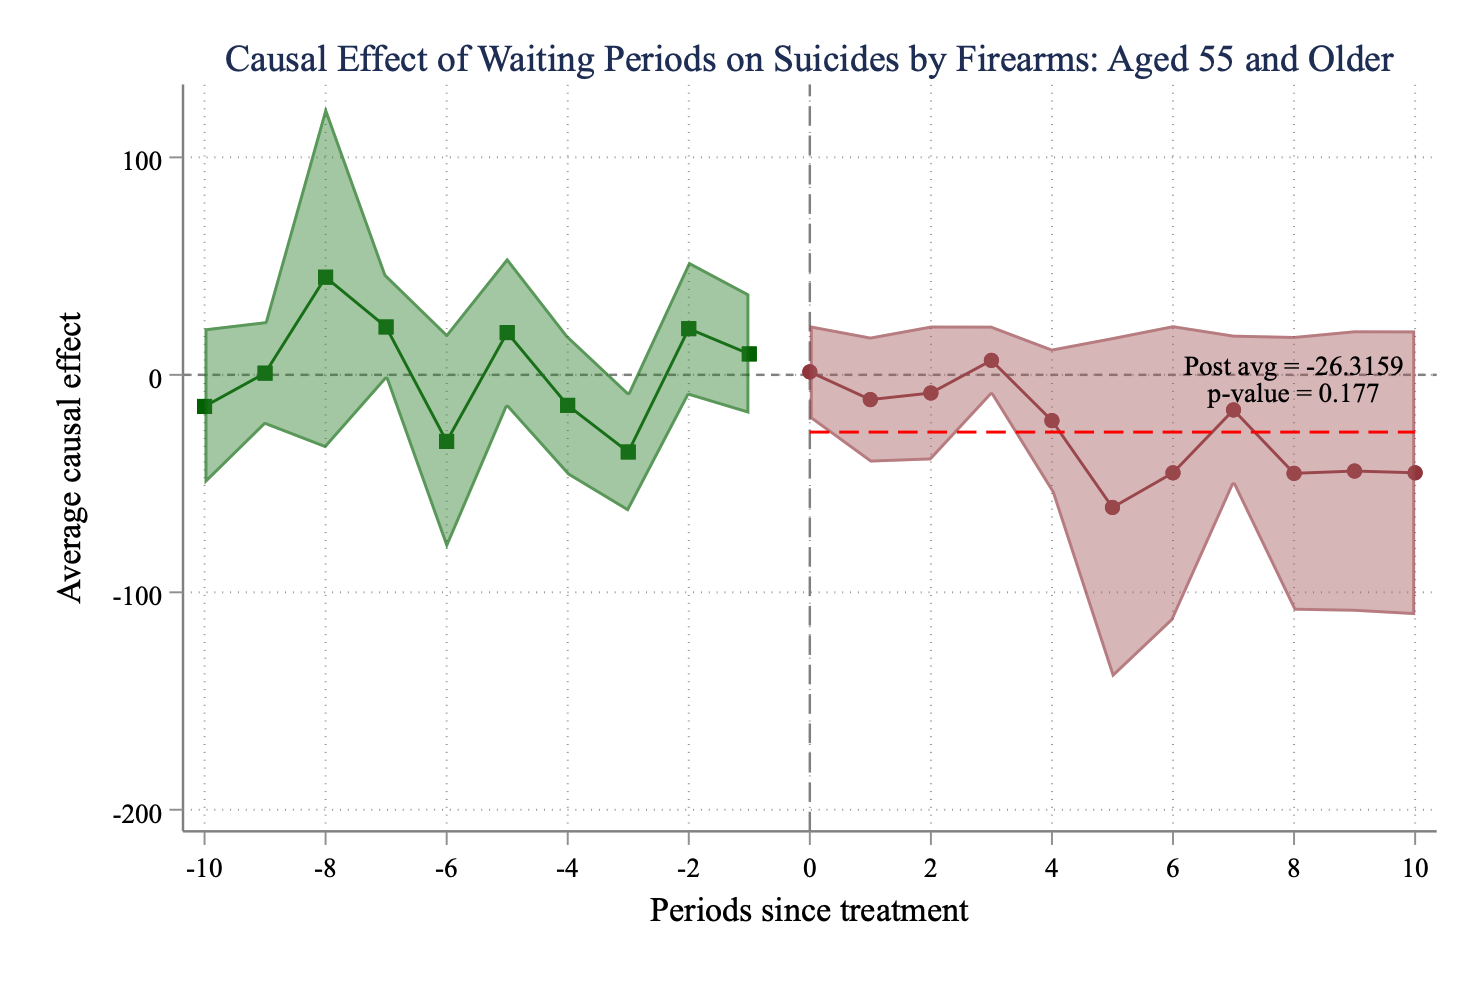
\includegraphics[width=0.8\textwidth]{figures/1037-csid-age_55p-fire-noNY.png}
    \begin{minipage}{\linewidth}
    \caption*{\footnotesize{
      \noindent\textit{Note:} This event study estimates the policy effect on older adults, a group at elevated suicide risk. Standard errors are bootstrapped and clustered at the state level. 


    }}
  \end{minipage}
\end{figure}

\pagebreak
\clearpage

\begin{figure}[htbp]
    \centering
    \caption{Effect of Waiting Periods on Firearm Suicide Rates Among White Individuals}
    \label{fig:firearm_suicide_DID_white}
    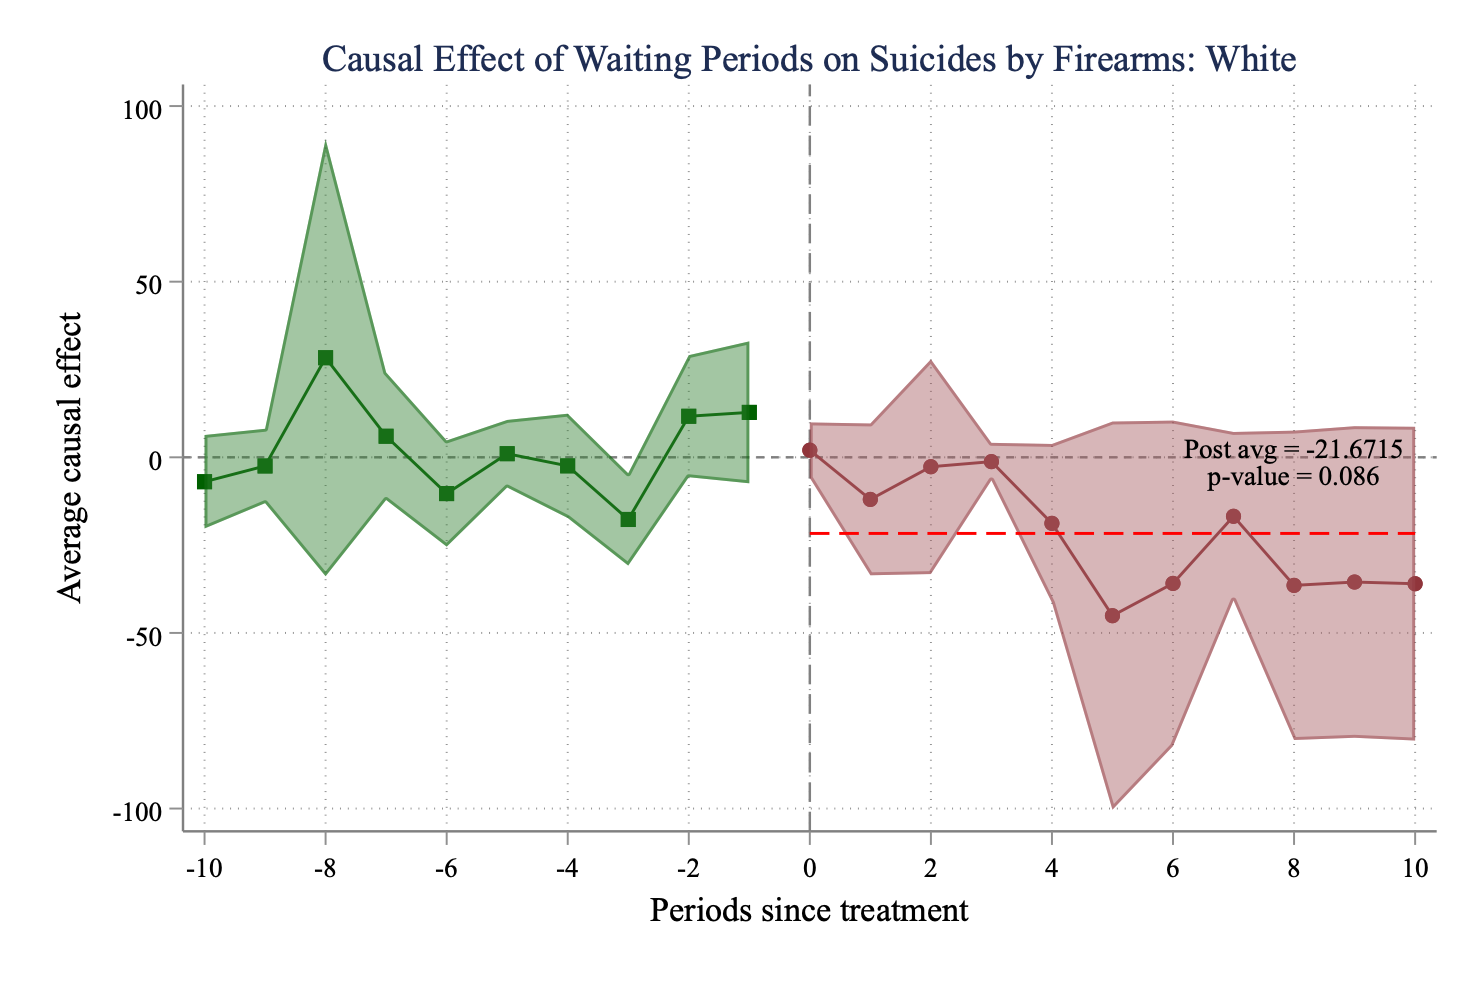
\includegraphics[width=0.8\textwidth]{figures/1038-csid-white-fire-noNY.png}
    \begin{minipage}{\linewidth}
    \caption*{\footnotesize{
      \noindent\textit{Note:} This figure examines firearm suicide trends for white individuals. Standard errors are bootstrapped and clustered at the state level. 
    }}
  \end{minipage}
\end{figure}

\pagebreak
\clearpage

\begin{figure}[htbp]
    \centering
    \caption{Effect of Waiting Periods on Non-Firearm Suicide Rates}
    \label{fig:firearm_suicide_DID_other}
    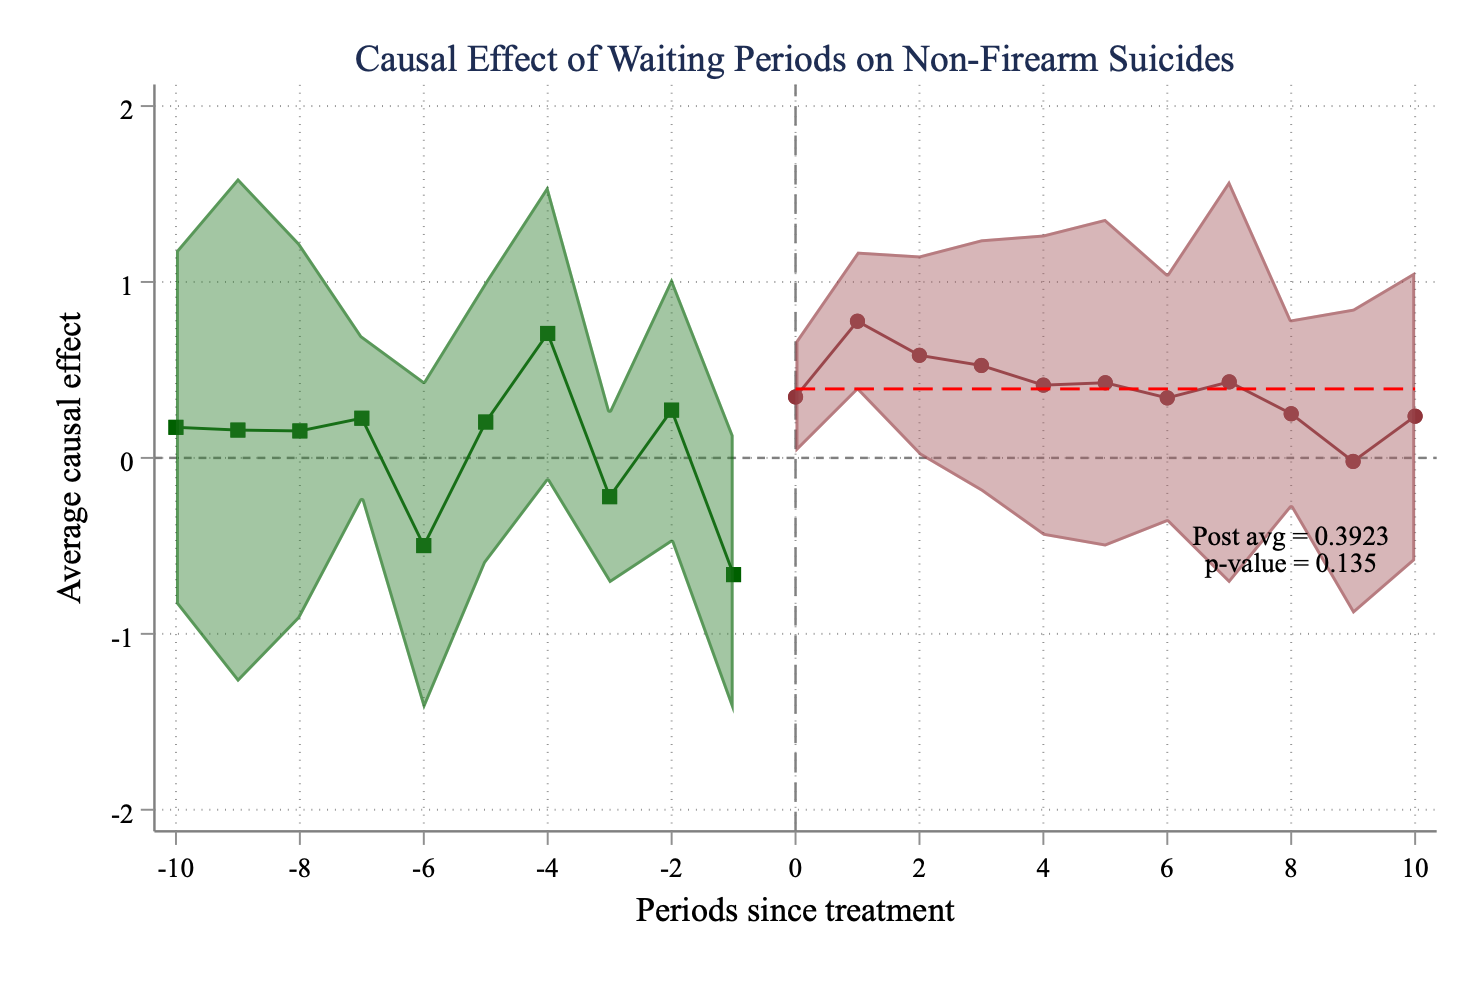
\includegraphics[width=0.8\textwidth]{figures/1039-csid-all-other-noNY.png}
    \begin{minipage}{\linewidth}
    \caption*{\footnotesize{
    This figure shows the dynamic effects of waiting period laws on all other suicide rates (non-firearm) across US counties. Each point represents the estimated difference in firearm suicide rates relative to the year of policy adoption (year 0), with 95\% confidence intervals. The absence of significant differences in pre-treatment periods supports the parallel trends assumption. Standard errors are bootstrapped and clustered at the state level. }}
  \end{minipage}
\end{figure}

\pagebreak
\clearpage

\begin{figure}[htbp]
    \centering
    \caption{Effect of Waiting Periods on Non-Firearm Suicide Rates Among Men}
    \label{fig:firearm_suicide_DID_other_men}
    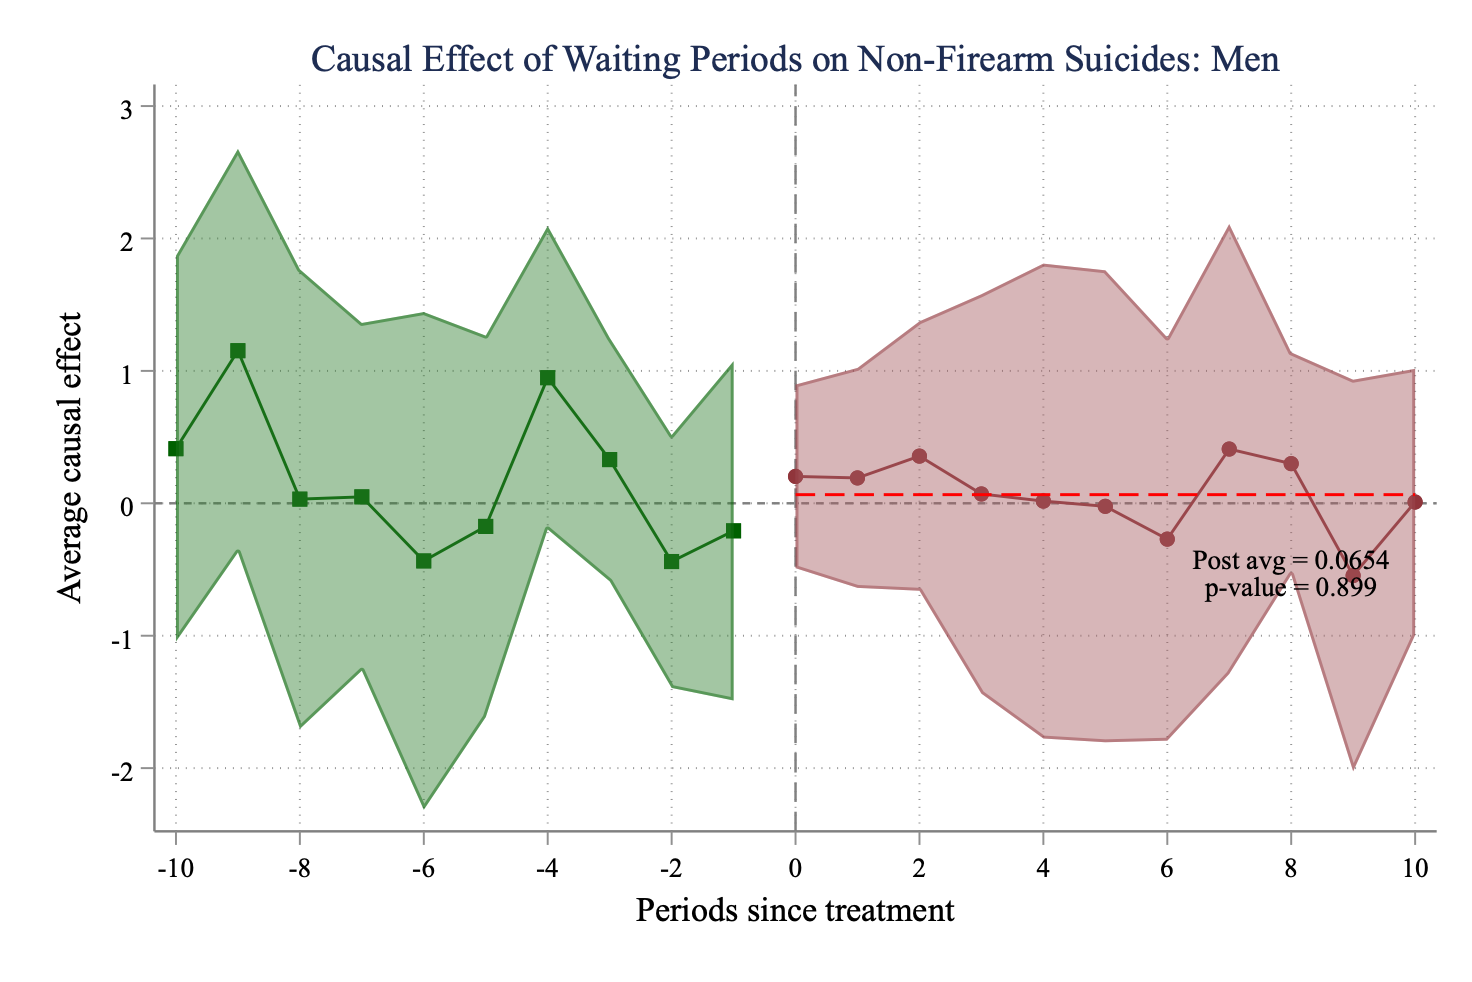
\includegraphics[width=0.8\textwidth]{figures/1040-csid-men-other-noNY.png}
    \begin{minipage}{\linewidth}
    \caption*{\footnotesize{
    This figure shows the dynamic effects of waiting period laws on all other suicide rates (non-firearm) across US counties among men. Each point represents the estimated difference in firearm suicide rates relative to the year of policy adoption (year 0), with 95\% confidence intervals. The absence of significant differences in pre-treatment periods supports the parallel trends assumption. Standard errors are bootstrapped and clustered at the state level.}}
  \end{minipage}
\end{figure}

\pagebreak
\clearpage

\begin{figure}[htbp]
    \centering
    \caption{Effect of Waiting Periods on Non-Firearm Suicide Rates Among Adults Aged 55+}
    \label{fig:firearm_suicide_DID_other_age55plus}
    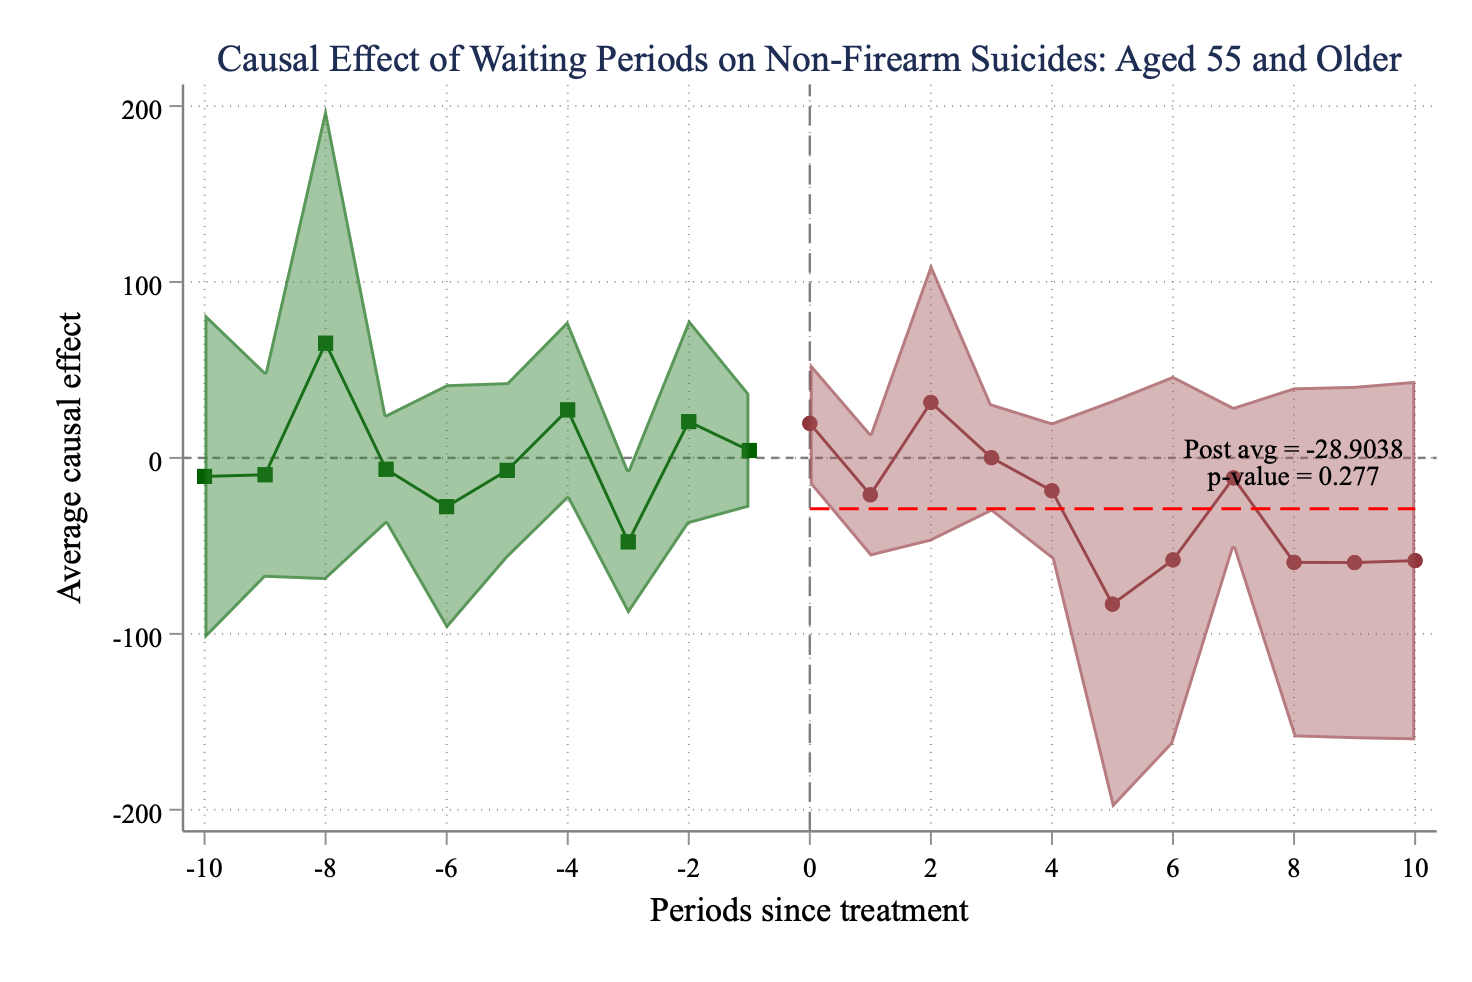
\includegraphics[width=0.8\textwidth]{figures/1041-csid-age_55p-other-noNY.png}
    \begin{minipage}{\linewidth}
    \caption*{\footnotesize{
    This figure shows the dynamic effects of waiting period laws on all other suicide rates (non-firearm) across US counties among adults aged 55+. Each point represents the estimated difference in firearm suicide rates relative to the year of policy adoption (year 0), with 95\% confidence intervals. The absence of significant differences in pre-treatment periods supports the parallel trends assumption. Standard errors are bootstrapped and clustered at the state level. }}
  \end{minipage}
\end{figure}

\pagebreak
\clearpage

\begin{figure}[htbp]
    \centering
    \caption{Effect of Waiting Periods on Non-Firearm Suicide Rates Among White Individuals}
    \label{fig:firearm_suicide_DID_other_white}
    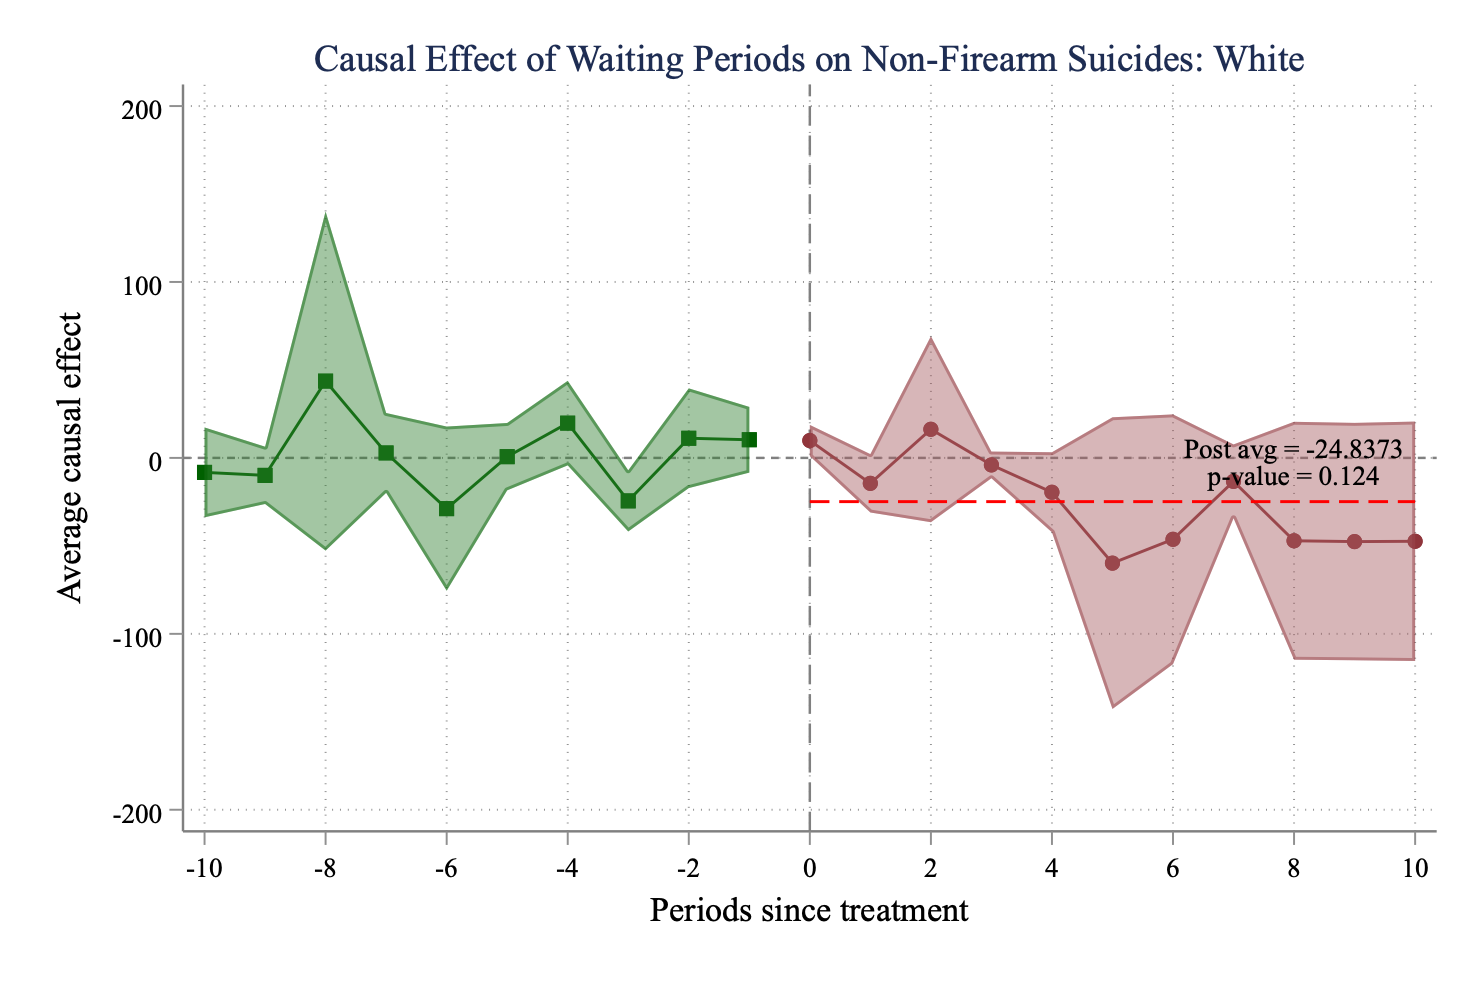
\includegraphics[width=0.8\textwidth]{figures/1042-csid-white-other-noNY.png}
    \begin{minipage}{\linewidth}
    \caption*{\footnotesize{
    This figure shows the dynamic effects of waiting period laws on all other suicide rates (non-firearm) across US counties among White individuals. Each point represents the estimated difference in firearm suicide rates relative to the year of policy adoption (year 0), with 95\% confidence intervals. The absence of significant differences in pre-treatment periods supports the parallel trends assumption. Standard errors are bootstrapped and clustered at the state level. }}
  \end{minipage}
\end{figure}


\pagebreak
\clearpage

\begin{figure}[htbp]
    \centering
    \caption{Estimated Effect of Waiting Periods on Overall Firearm Suicide Rates: Out of Treatment Sample}
    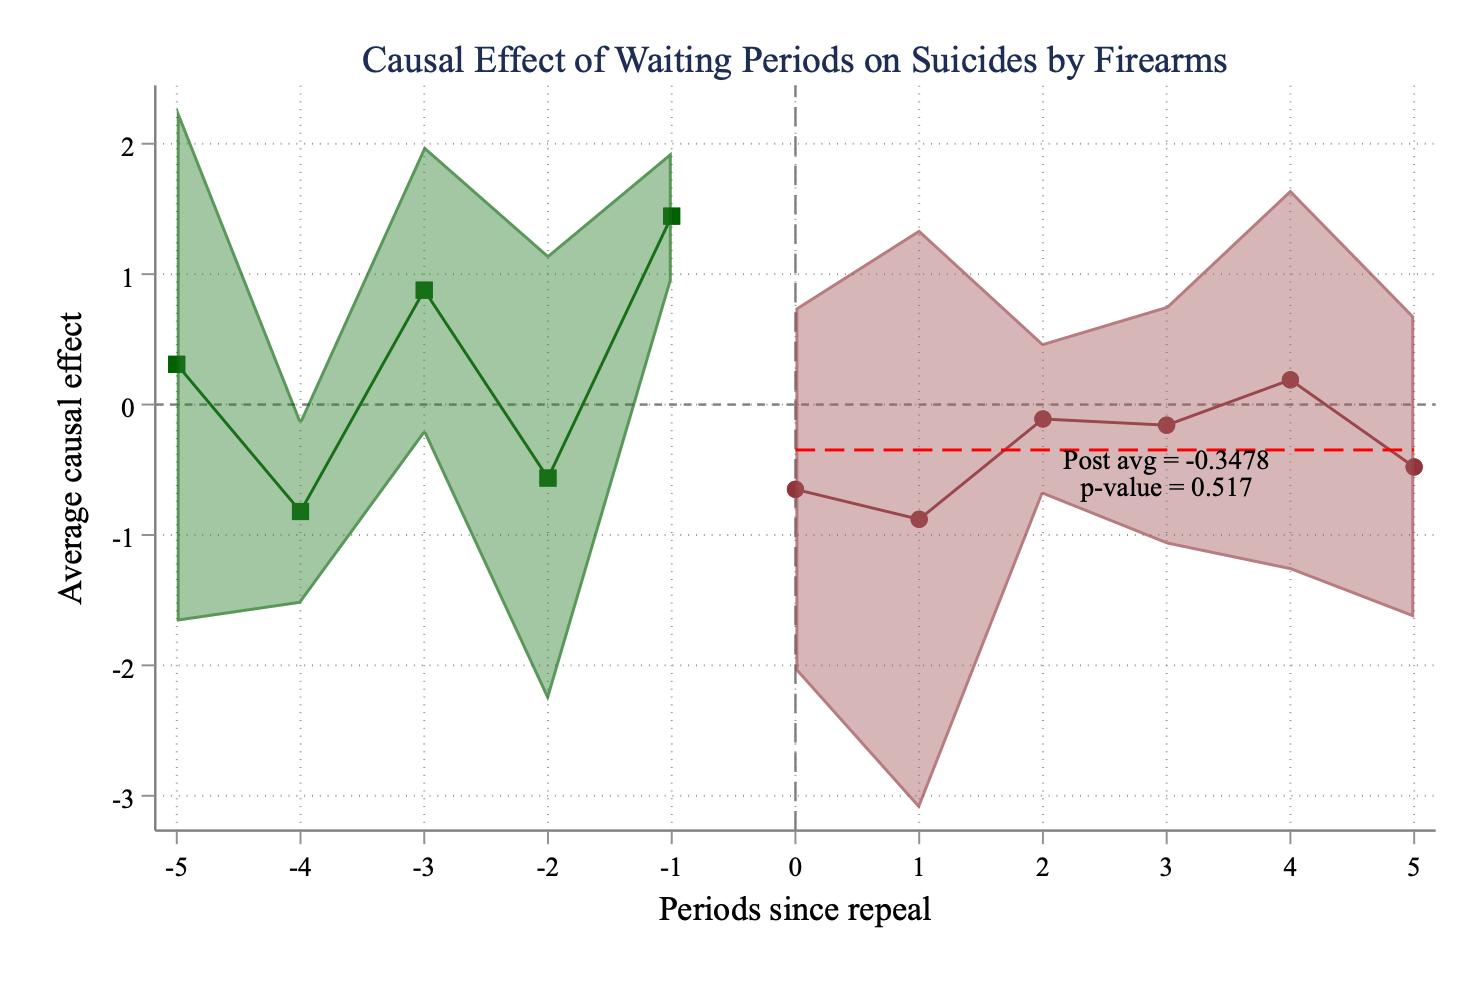
\includegraphics[width=0.8\textwidth]{figures/1008-csid-outsample-fire.png}
    \label{fig:firearm_suicide_DID_overall-out}

    \begin{minipage}{\linewidth}
    \caption*{\footnotesize{
      \noindent\textit{Note:} This figure shows the dynamic effects of waiting period laws on firearm suicide rates across US counties using a sample of states that move out of treatment. The sample is composed of states that experience either one policy transition from treatment to no-treatment, or always treated, yielding 23 states (13 treatment, 13 control). Each point represents the estimated difference in firearm suicide rates relative to the year of policy adoption (year 0), with 95\% confidence intervals. Standard errors are bootstrapped and clustered at the state level. 
    }}
  \end{minipage}
\end{figure}

\pagebreak
\clearpage

\begin{figure}[htbp]
    \centering
    \caption{Effect of Waiting Periods on Firearm Suicide Rates Among Men: Out of Treatment Sample}
    \label{fig:firearm_suicide_DID_men-out}
    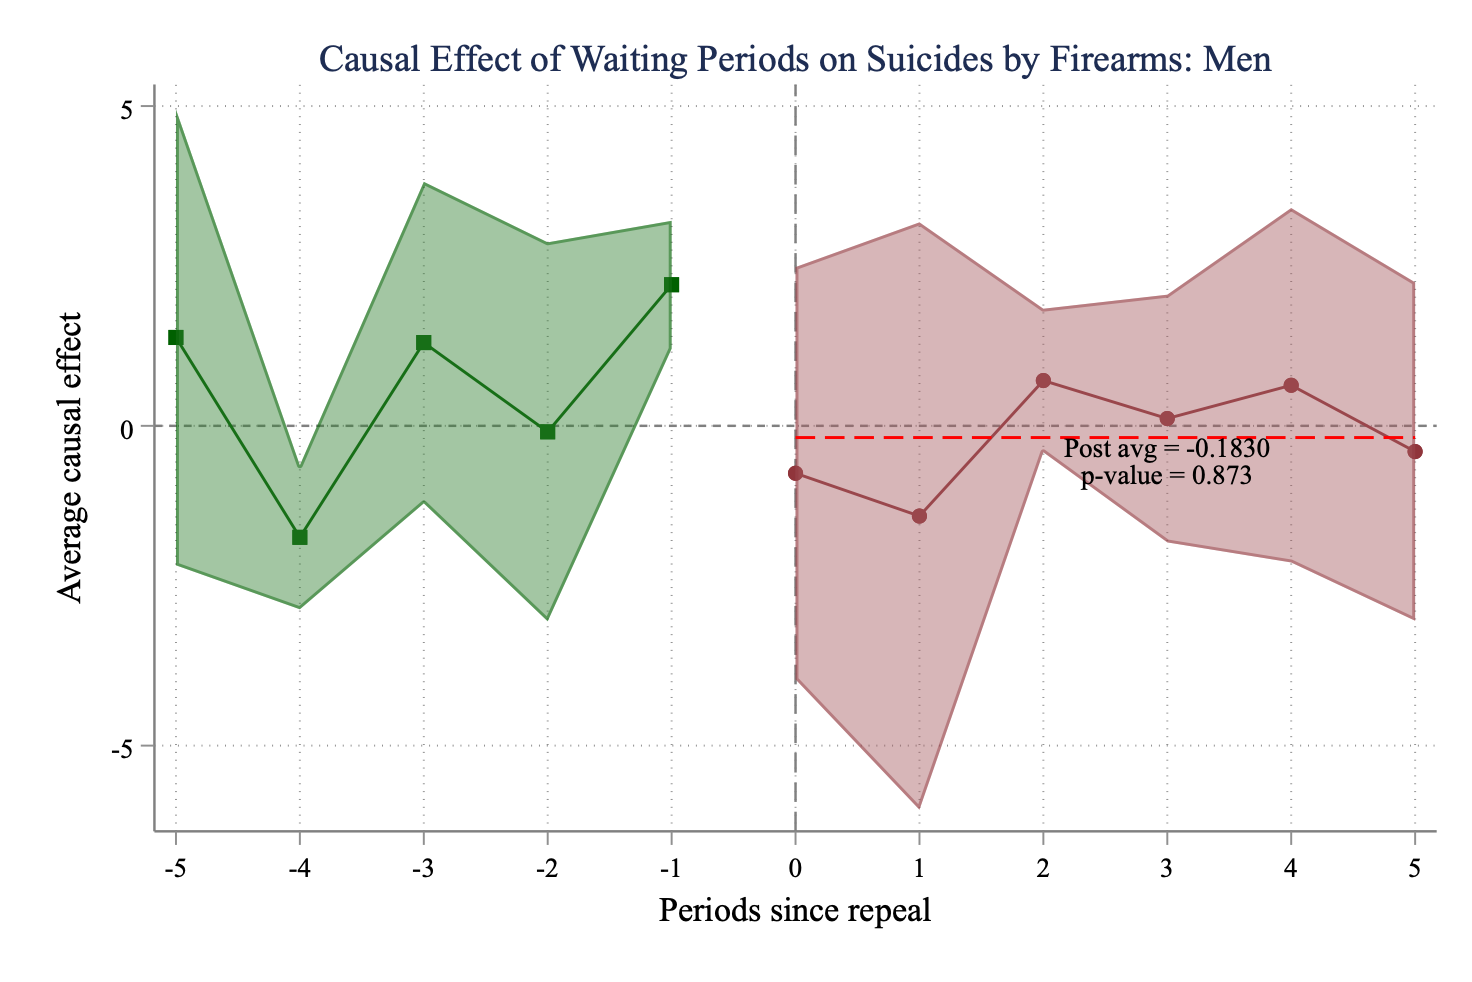
\includegraphics[width=0.8\textwidth]{figures/1009-csid-men-outsample-fire.png}
    \begin{minipage}{\linewidth}
    \caption*{\footnotesize{
      \noindent\textit{Note:} This figure focuses on the male population using a sample of states that move out of treatment, showing how waiting period laws affect firearm suicide rates for men specifically. The sample includes 23 states (13 treatment, 13 control) that experience either one policy transition from treatment to no-treatment, or always treated. Standard errors are bootstrapped and clustered at the state level. 
    }}
  \end{minipage}
\end{figure}

\pagebreak
\clearpage

\begin{figure}[htbp]
    \centering
    \caption{Effect of Waiting Periods on Firearm Suicide Rates Among Adults Aged 55+: Out of Treatment Sample}
    \label{fig:firearm_suicide_DID_older-out}
    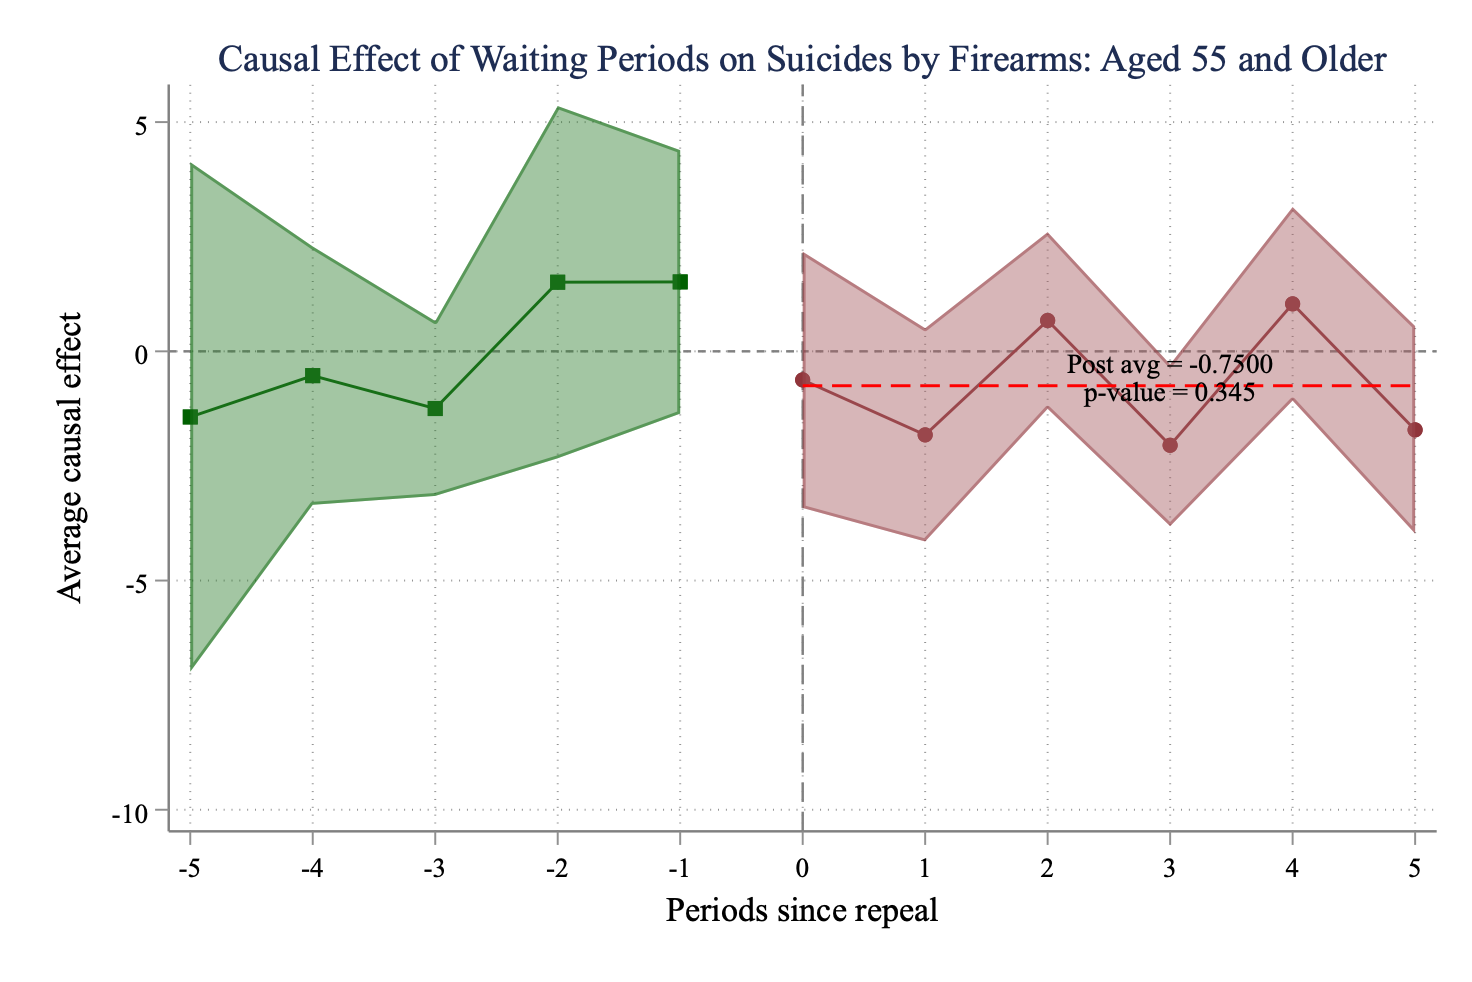
\includegraphics[width=0.8\textwidth]{figures/1010-csid-age_55p-outsample-fire.png}
    \begin{minipage}{\linewidth}
    \caption*{\footnotesize{
      \noindent\textit{Note:} This event study estimates the policy effect on older adults using a sample of states that move out of treatment, focusing on a group at elevated suicide risk. The sample comprises 23 states (13 treatment, 13 control) that experience either one policy transition from treatment to no-treatment, or always treated. Standard errors are bootstrapped and clustered at the state level. 
    }}
  \end{minipage}
\end{figure}

\pagebreak
\clearpage

\begin{figure}[htbp]
    \centering
    \caption{Effect of Waiting Periods on Firearm Suicide Rates Among White Individuals: Out of Treatment Sample}
    \label{fig:firearm_suicide_DID_white-out}
    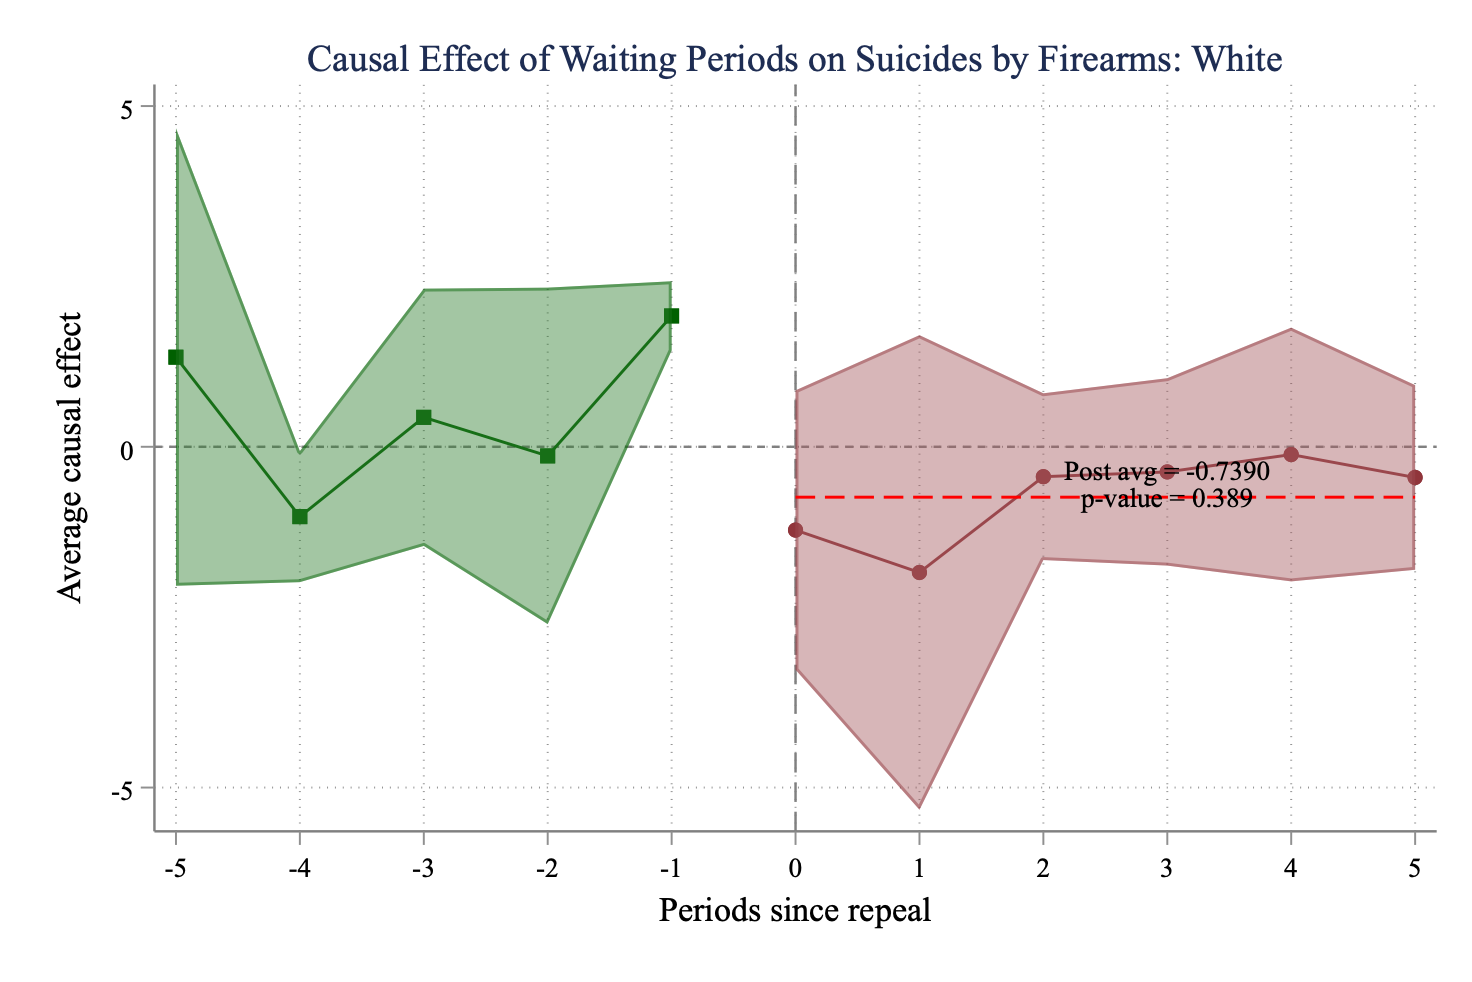
\includegraphics[width=0.8\textwidth]{figures/1011-csid-white-outsample-fire.png}
    \begin{minipage}{\linewidth}
    \caption*{\footnotesize{
      \noindent\textit{Note:} This figure examines firearm suicide trends for white individuals using a sample of states that move out of treatment. The sample includes 23 states (13 treatment, 13 control) that experience either one policy transition from treatment to no-treatment, or always treated. Standard errors are bootstrapped and clustered at the state level. 
    }}
  \end{minipage}
\end{figure}

\pagebreak
\clearpage

\begin{figure}[htbp]
    \centering
    \caption{Effect of Waiting Periods on Non-Firearm Suicide Rates: Out of Treatment Sample}
    \label{fig:firearm_suicide_DID_other-out}
    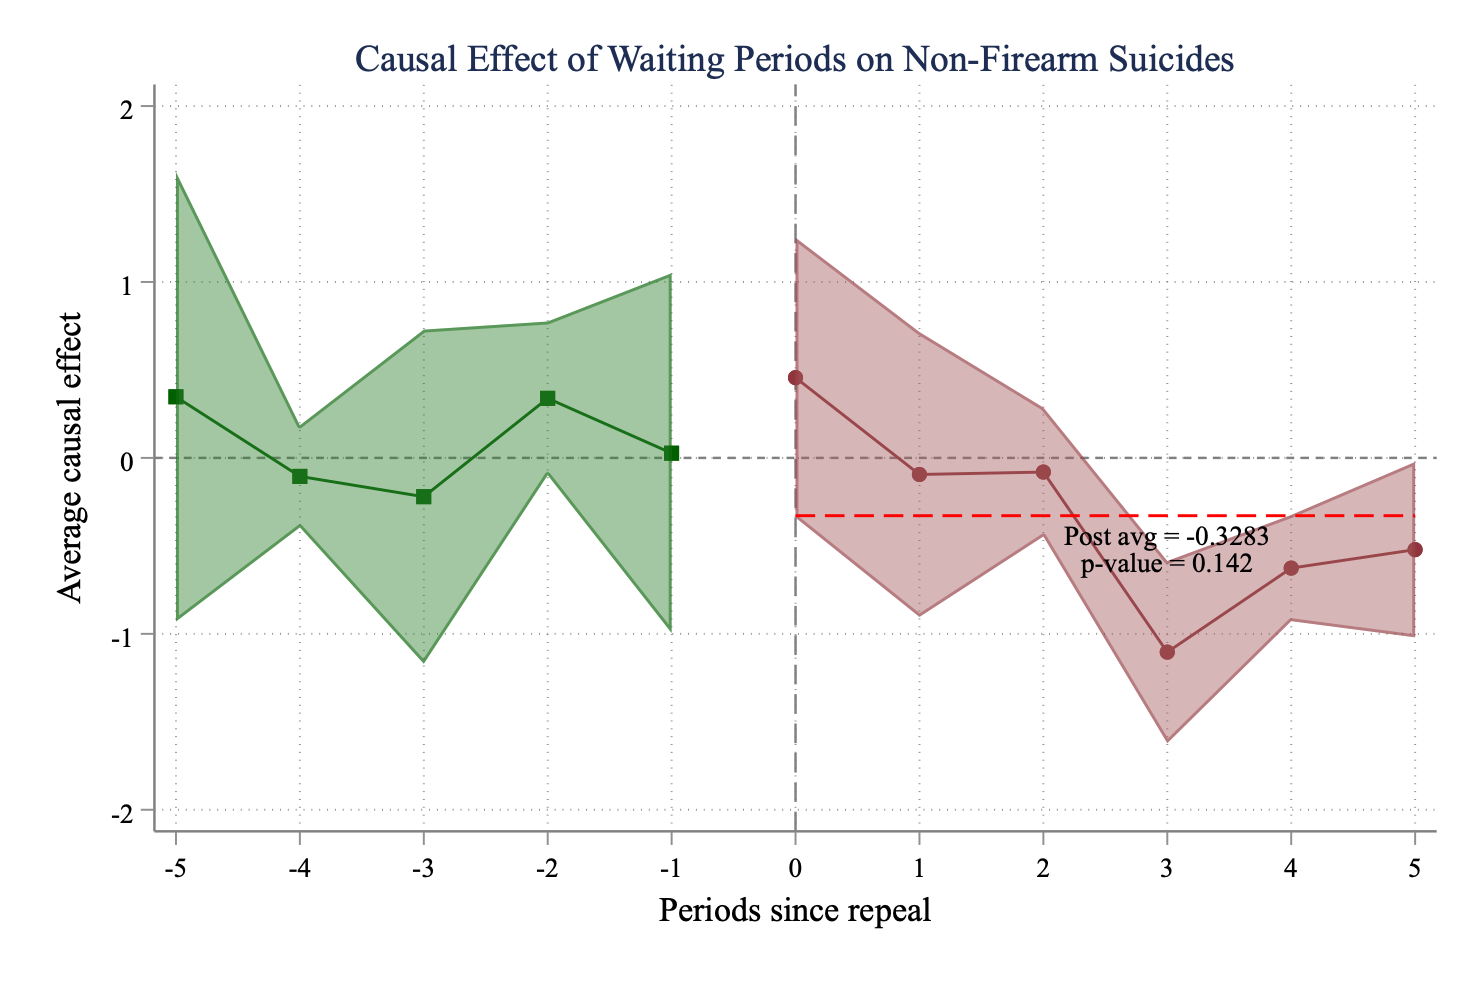
\includegraphics[width=0.8\textwidth]{figures/1012-csid-all-outsample-other.png}
    \begin{minipage}{\linewidth}
    \caption*{\footnotesize{
    This figure shows the dynamic effects of waiting period laws on all other suicide rates (non-firearm) across US counties using a sample of states that move out of treatment. The sample comprises 23 states (13 treatment, 13 control) that experience either one policy transition from treatment to no-treatment, or always treated. Standard errors are bootstrapped and clustered at the state level. }}
  \end{minipage}
\end{figure}

\pagebreak
\clearpage

\begin{figure}[htbp]
    \centering
    \caption{Effect of Waiting Periods on Non-Firearm Suicide Rates Among Men: Out of Treatment Sample}
    \label{fig:firearm_suicide_DID_other_men-out}
    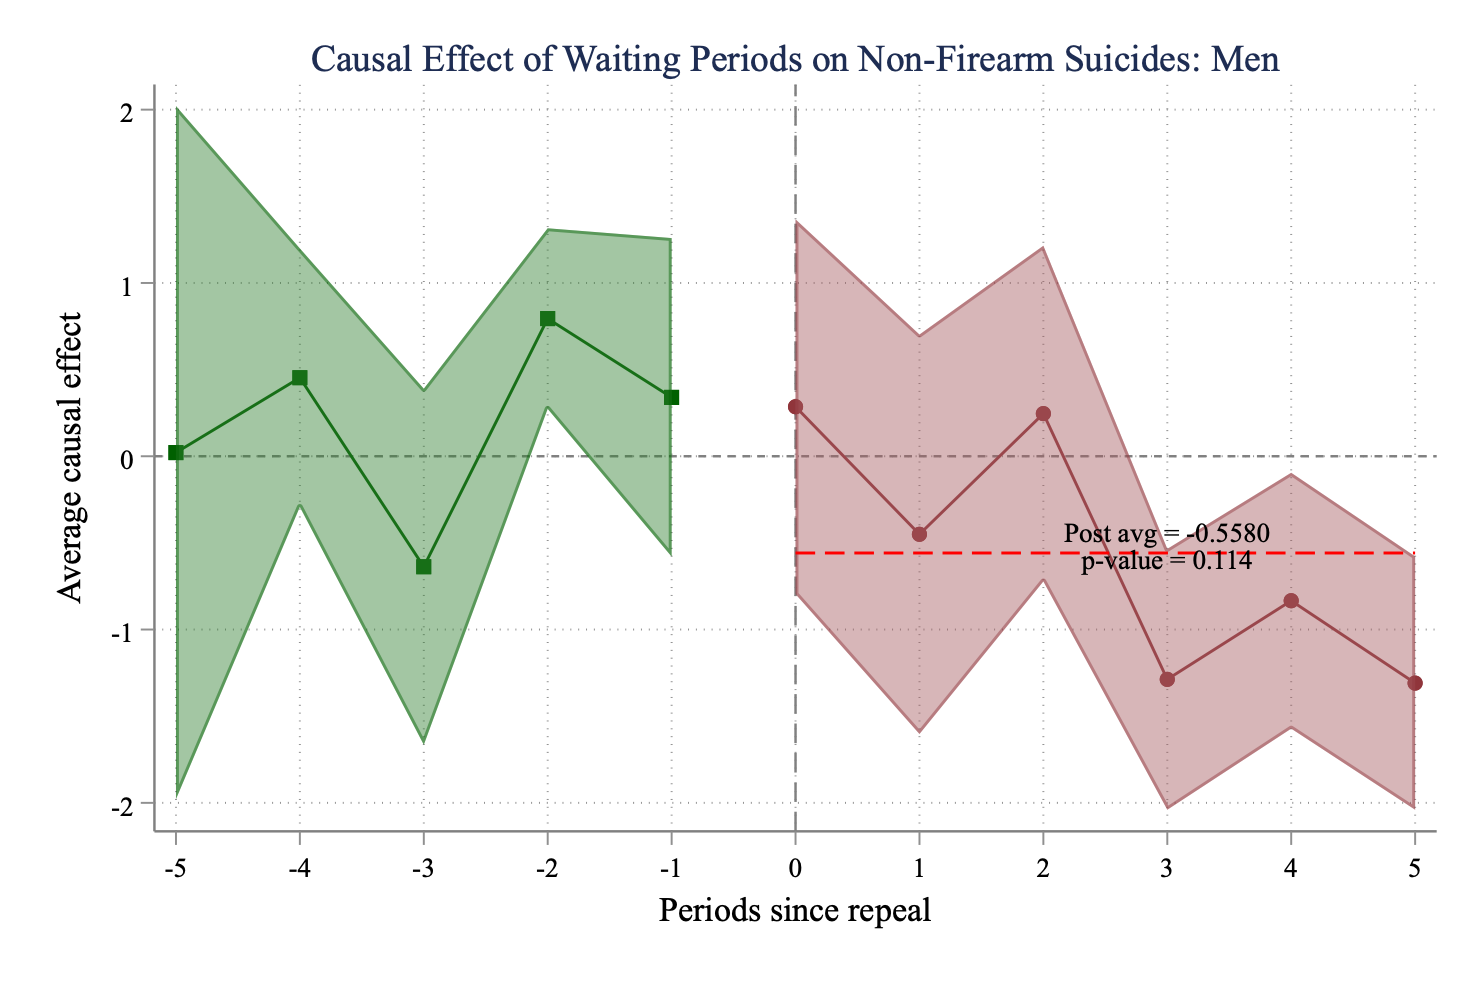
\includegraphics[width=0.8\textwidth]{figures/1013-csid-outsample-men-other.png}
    \begin{minipage}{\linewidth}
    \caption*{\footnotesize{
    This figure shows the dynamic effects of waiting period laws on all other suicide rates (non-firearm) across US counties among men using a sample of states that move out of treatment. The sample includes 23 states (13 treatment, 13 control) that experience either one policy transition from treatment to no-treatment, or always treated. Standard errors are bootstrapped and clustered at the state level. }}
  \end{minipage}
\end{figure}

\pagebreak
\clearpage

\begin{figure}[htbp]
    \centering
    \caption{Effect of Waiting Periods on Non-Firearm Suicide Rates Among Adults Aged 55+: Out of Treatment Sample}
    \label{fig:firearm_suicide_DID_other_age55plus-out}
    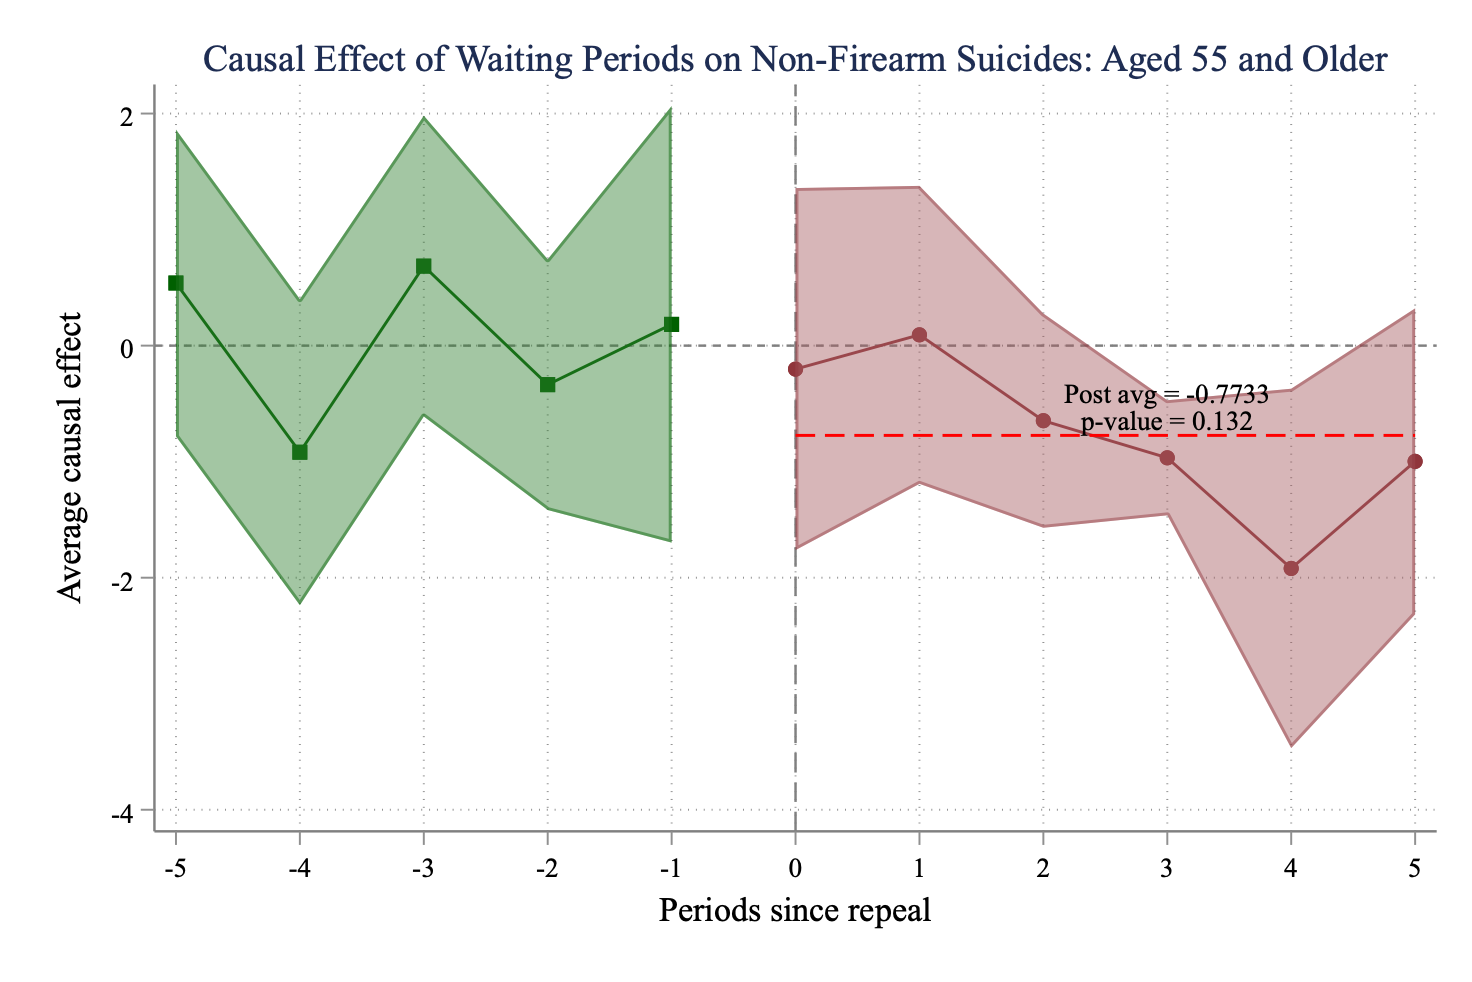
\includegraphics[width=0.8\textwidth]{figures/1014-csid-outsample-age_55p-other.png}
    \begin{minipage}{\linewidth}
    \caption*{\footnotesize{
    This figure shows the dynamic effects of waiting period laws on all other suicide rates (non-firearm) across US counties among adults aged 55+ using a sample of states that move out of treatment. The sample comprises 23 states (13 treatment, 13 control) that experience either one policy transition from treatment to no-treatment, or always treated. Standard errors are bootstrapped and clustered at the state level. }}
  \end{minipage}
\end{figure}

\pagebreak
\clearpage

\begin{figure}[htbp]
    \centering
    \caption{Effect of Waiting Periods on Non-Firearm Suicide Rates Among White Individuals: Out of Treatment Sample}
    \label{fig:firearm_suicide_DID_other_white-out}
    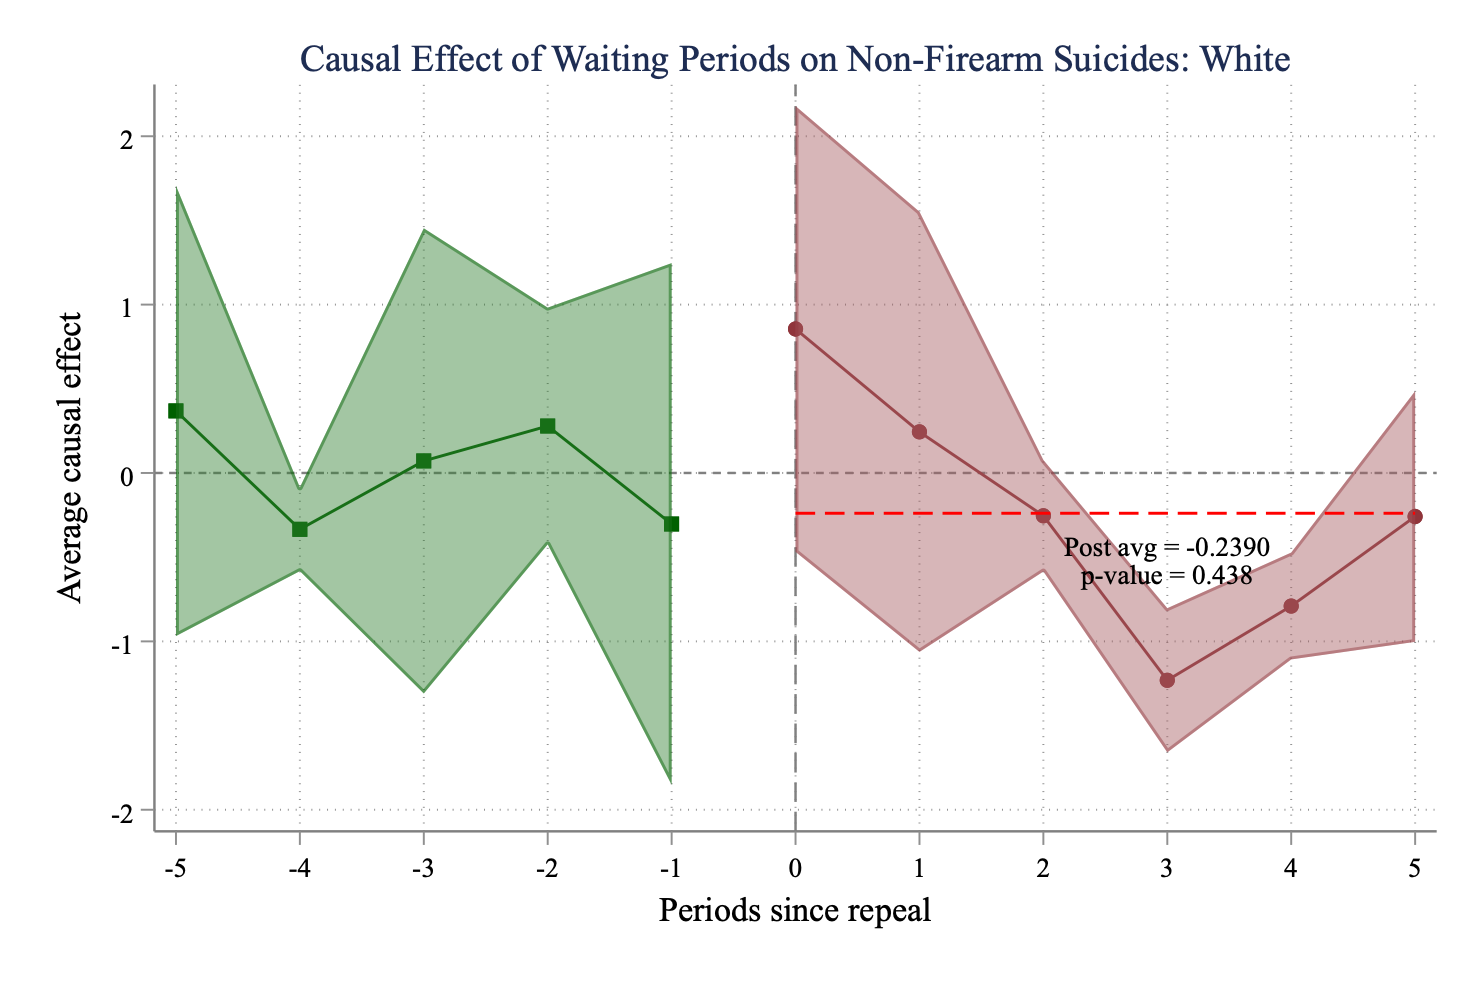
\includegraphics[width=0.8\textwidth]{figures/1015-csid-outsample-white-other.png}
    \begin{minipage}{\linewidth}
    \caption*{\footnotesize{
    This figure shows the dynamic effects of waiting period laws on all other suicide rates (non-firearm) across US counties among White individuals using a sample of states that move out of treatment. The sample includes 23 states (13 treatment, 13 control) that experience either one policy transition from treatment to no-treatment, or always treated. Standard errors are bootstrapped and clustered at the state level. }}
  \end{minipage}
\end{figure}

\pagebreak
\clearpage

\begin{figure}[htbp]
    \centering
    \caption{Effect of Waiting Periods on Firearm Suicide Rates: Different Types of Estimators}
    \label{fig:1033-all-estimators}
    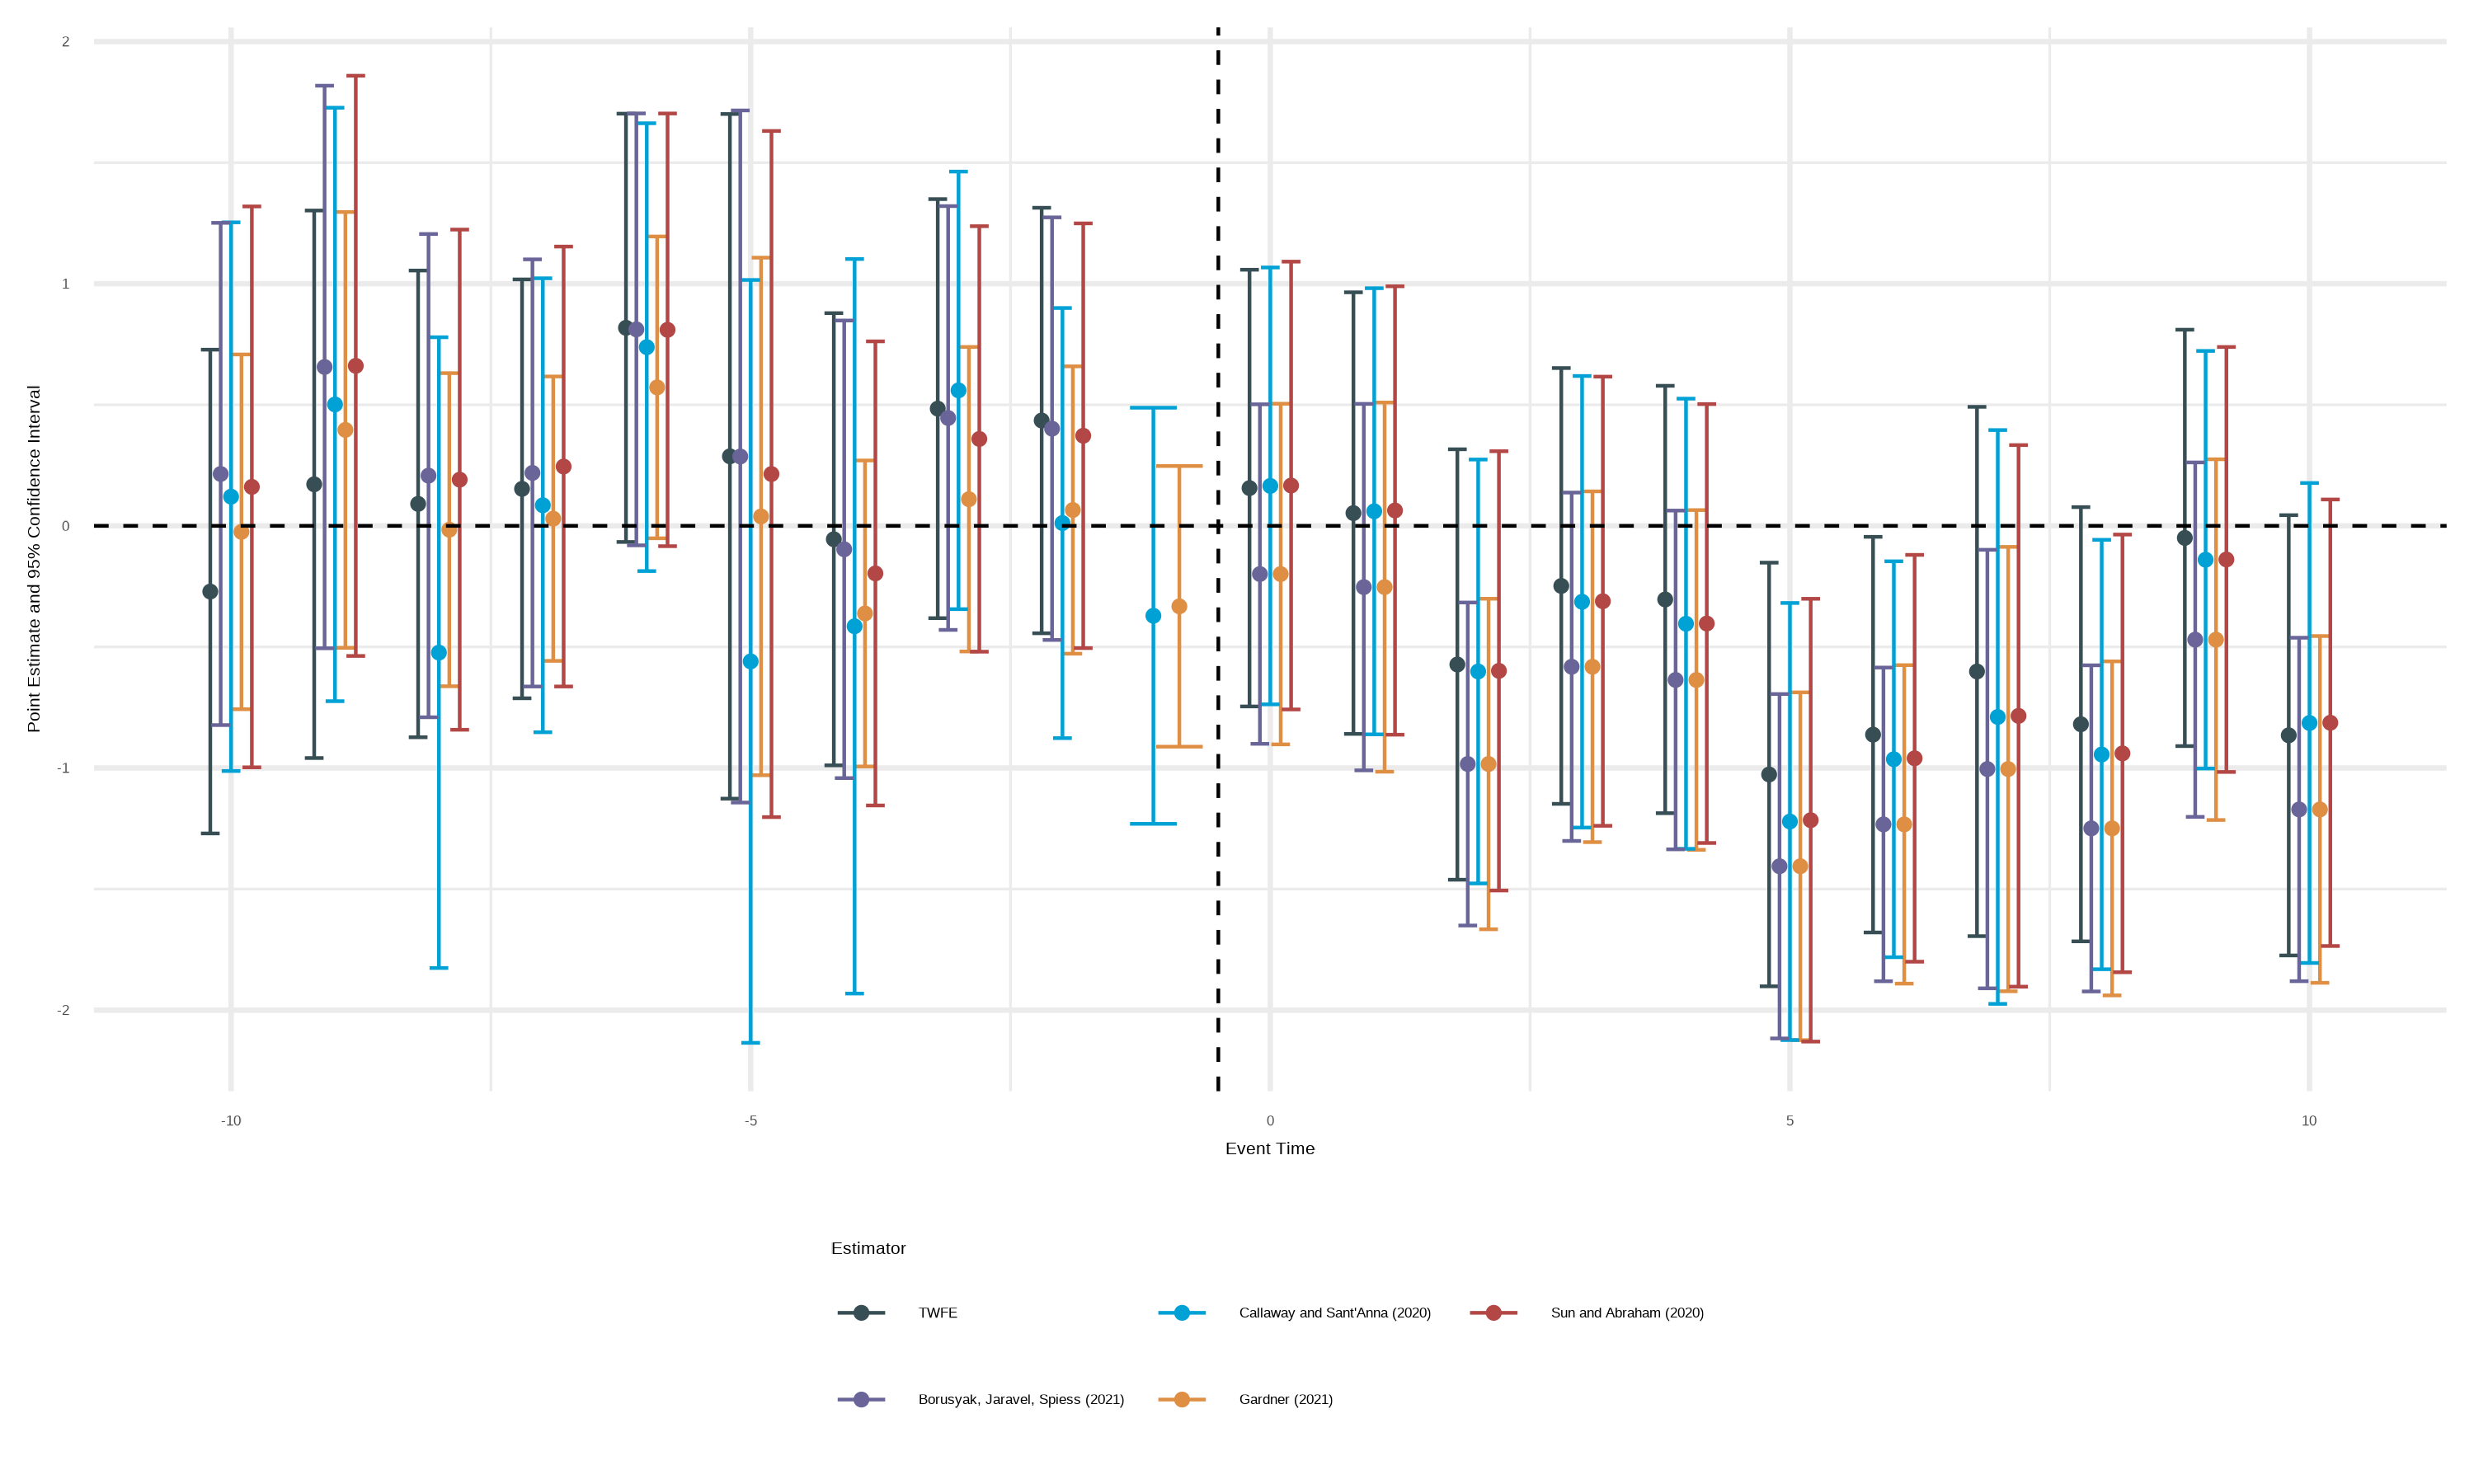
\includegraphics[width=0.8\textwidth]{figures/1033-all-estimators.png}
    \begin{minipage}{\linewidth}
    \caption*{\footnotesize{
    This figure shows the dynamic effects of waiting period laws on firearm suicide rates across US counties using multiple DiD estimators.}}
  \end{minipage}
\end{figure}


\pagebreak
\clearpage
%%%%%%%%%%%%%%%%%%%%%%%%%%%%%%%%%%%%
% Tables
%%%%%%%%%%%%%%%%%%%%%%%%%%%%%%%%%%%%
% Table 1

\clearpage
\pagebreak

\begin{table}
\centering
\caption{Summary Statistics for County-Year Data}\label{tab01:sum}
\centering
\begin{tabular}[t]{lrrrrr}
\toprule
  & Mean & SD & Min & Max & N\\
\midrule
Total Suicide Rate (per 100k) & \num{13.64} & \num{14.14} & \num{0.00} & \num{575.54} & 80,313\\
Firearm Suicide Rate (per 100k) & \num{8.45} & \num{11.00} & \num{0.00} & \num{431.65} & 80,313\\
Men's Firearm Suicide Rate (per 100k) & \num{14.86} & \num{19.92} & \num{0.00} & \num{677.97} & 80,313\\
Firearm Suicide Rate Aged 55+ (per 100k) & \num{24.99} & \num{221.42} & \num{0.00} & \num{33,333.33} & 80,313\\
White Individuals' Firearm Suicide Rate (per 100k) & \num{16.11} & \num{97.85} & \num{0.00} & \num{9,000.00} & 80,313\\
Non-Firearm Suicide Rate (per 100k) & \num{5.19} & \num{7.55} & \num{0.00} & \num{358.42} & 80,313\\
Female Population Share & \num{0.50} & \num{0.02} & \num{0.28} & \num{0.62} & 80,313\\
\bottomrule
\end{tabular}
\vspace{0.2em}
\begin{minipage}{0.95\linewidth}
\footnotesize\emph{Notes}: Data come from the National Vital Statistics System (NVSS), 1959--2019. Suicide rates are expressed per 100{,}000 population. ``Female Population Share'', ``College Educated'', and ``Below Poverty Line'' are proportions. SD denotes standard deviation. N is the number of county--year observations (80{,}313).
\end{minipage}
\end{table}


\clearpage
\pagebreak

\begin{landscape}
\begin{table}
\centering
\caption{Comparison of Treated and Control Groups}
\centering
\begin{tabular}[t]{lrrrrrr}
\toprule
\multicolumn{1}{c}{ } & \multicolumn{2}{c}{Control (N=60,300)} & \multicolumn{2}{c}{Treated (N=20,013)} & \multicolumn{2}{c}{ } \\
\cmidrule(l{3pt}r{3pt}){2-3} \cmidrule(l{3pt}r{3pt}){4-5}
  & Mean & Std. Dev. & Mean & Std. Dev. & Diff. in Means & Std. Error\\
\midrule
Total Suicide Rate (per 100k) & \num{13.8} & \num{15.2} & \num{13.3} & \num{10.2} & \num{-0.4} & \num{0.1}\\
Firearm Suicide Rate (per 100k) & \num{8.7} & \num{11.8} & \num{7.6} & \num{7.9} & \num{-1.1} & \num{0.1}\\
Men's Firearm Suicide Rate (per 100k) & \num{15.3} & \num{21.5} & \num{13.5} & \num{14.1} & \num{-1.9} & \num{0.1}\\
Firearm Suicide Rate Aged 55+ (per 100k) & \num{27.1} & \num{246.0} & \num{18.6} & \num{119.7} & \num{-8.5} & \num{1.3}\\
White Individuals' Firearm Suicide Rate (per 100k) & \num{17.3} & \num{99.5} & \num{12.6} & \num{92.6} & \num{-4.7} & \num{0.8}\\
Non-Firearm Suicide Rate (per 100k) & \num{5.0} & \num{8.1} & \num{5.7} & \num{5.6} & \num{0.6} & \num{0.1}\\
Female Population Share & \num{0.5} & \num{0.0} & \num{0.5} & \num{0.0} & \num{0.0} & \num{0.0}\\
College Educated (\%) & \num{0.1} & \num{1.4} & \num{0.1} & \num{0.8} & \num{0.0} & \num{0.0}\\
Below Poverty Line (\%) & \num{0.3} & \num{2.4} & \num{0.1} & \num{1.3} & \num{-0.2} & \num{0.0}\\
\bottomrule
\end{tabular}
\end{table}
    
\end{landscape}

\clearpage
\pagebreak

\begin{table}[H]
\centering\centering
\caption{Treatment Cohorts by State \label{tab:tab-01}}
\centering
\begin{tabular}[t]{>{}lcc>{\raggedright\arraybackslash}p{10em}}
\toprule
Treatment Cohort & State Count & Percent of States & State Abbreviations\\
\midrule
\textbf{1965 Cohort} & 2 & 3.92\% & CA, CT\\
\textbf{1966 Cohort} & 1 & 1.96\% & MD\\
\textbf{1967 Cohort} & 1 & 1.96\% & IL\\
\textbf{1969 Cohort} & 1 & 1.96\% & WA\\
\textbf{1973 Cohort} & 3 & 5.88\% & IN, OR, PA\\
\addlinespace
\textbf{1976 Cohort} & 1 & 1.96\% & WI\\
\textbf{1977 Cohort} & 1 & 1.96\% & MN\\
\textbf{1979 Cohort} & 1 & 1.96\% & NJ\\
\textbf{1988 Cohort} & 1 & 1.96\% & HI\\
\textbf{1991 Cohort} & 1 & 1.96\% & FL\\
\addlinespace
\textbf{1994 Cohort} & 19 & 37.25\% & AK, AZ, AR, GA, ID, KS, KY, LA, ME, MS, MT, NH, NM, ND, OK, TX, VT, WV, WY\\
\textbf{Always Treated} & 5 & 9.8\% & AL, DC, RI, SD, TN\\
\textbf{Never Treated} & 14 & 27.45\% & CO, DE, IA, MA, MI, MO, NE, NV, NY, NC, OH, SC, UT, VA\\
\midrule
\textbf{Total} & 51 & 100\% & \\
\bottomrule
\end{tabular}
\begin{minipage}{0.95\linewidth}
\footnotesize\emph{Notes}: Data from RAND State Firearm Law Database. Always treated are the states that had a waiting period law in place before at 1959, the first year of vital statistics data that is available. They include states that might have 
moved to a less restrictive waiting periods or abolished them.
\end{minipage}
\end{table}
